\documentclass[reqno,10pt,a4paper,oneside]{amsart}

\usepackage{amsmath,geometry}
\usepackage{amssymb,mathpartir,mathtools}
\usepackage{latexsym}
\usepackage{amsthm}
 \usepackage[show]{ed}
\usepackage{leftidx}
\usepackage{tikz}
\usepackage[all]{xy}
\newcommand{\xycenter}[1]{\vcenter{\hbox{\xymatrix{#1}}}}
\SelectTips{cm}{}
% Proof trees
\message{<Paul Taylor's Proof Trees, 2 August 1996>}
%% Build proof tree for Natural Deduction, Sequent Calculus, etc.
%% WITH SHORTENING OF PROOF RULES!
%% Paul Taylor, begun 10 Oct 1989
%% *** THIS IS ONLY A PRELIMINARY VERSION AND THINGS MAY CHANGE! ***
%%
%% 2 Aug 1996: fixed \mscount and \proofdotnumber
%%
%%      \prooftree
%%              hyp1            produces:
%%              hyp2
%%              hyp3            hyp1    hyp2    hyp3
%%      \justifies              -------------------- rulename
%%              concl                   concl
%%      \thickness=0.08em
%%      \shiftright 2em
%%      \using
%%              rulename
%%      \endprooftree
%%
%% where the hypotheses may be similar structures or just formulae.
%%
%% To get a vertical string of dots instead of the proof rule, do
%%
%%      \prooftree                      which produces:
%%              [hyp]
%%      \using                                  [hyp]
%%              name                              .
%%      \proofdotseparation=1.2ex                 .name
%%      \proofdotnumber=4                         .
%%      \leadsto                                  .
%%              concl                           concl
%%      \endprooftree
%%
%% Within a prooftree, \[ and \] may be used instead of \prooftree and
%% \endprooftree; this is not permitted at the outer level because it
%% conflicts with LaTeX. Also,
%%      \Justifies
%% produces a double line. In LaTeX you can use \begin{prooftree} and
%% \end{prootree} at the outer level (however this will not work for the inner
%% levels, but in any case why would you want to be so verbose?).
%%
%% All of of the keywords except \prooftree and \endprooftree are optional
%% and may appear in any order. They may also be combined in \newcommand's
%% eg "\def\Cut{\using\sf cut\thickness.08em\justifies}" with the abbreviation
%% "\prooftree hyp1 hyp2 \Cut \concl \endprooftree". This is recommended and
%% some standard abbreviations will be found at the end of this file.
%%
%% \thickness specifies the breadth of the rule in any units, although
%% font-relative units such as "ex" or "em" are preferable.
%% It may optionally be followed by "=".
%% \proofrulebreadth=.08em or \setlength\proofrulebreadth{.08em} may also be
%% used either in place of \thickness or globally; the default is 0.04em.
%% \proofdotseparation and \proofdotnumber control the size of the
%% string of dots
%%
%% If proof trees and formulae are mixed, some explicit spacing is needed,
%% but don't put anything to the left of the left-most (or the right of
%% the right-most) hypothesis, or put it in braces, because this will cause
%% the indentation to be lost.
%%
%% By default the conclusion is centered wrt the left-most and right-most
%% immediate hypotheses (not their proofs); \shiftright or \shiftleft moves
%% it relative to this position. (Not sure about this specification or how
%% it should affect spreading of proof tree.)
%
% global assignments to dimensions seem to have the effect of stretching
% diagrams horizontally.
%
%%==========================================================================

\def\introrule{{\cal I}}\def\elimrule{{\cal E}}%%
\def\andintro{\using{\land}\introrule\justifies}%%
\def\impelim{\using{\Rightarrow}\elimrule\justifies}%%
\def\allintro{\using{\forall}\introrule\justifies}%%
\def\allelim{\using{\forall}\elimrule\justifies}%%
\def\falseelim{\using{\bot}\elimrule\justifies}%%
\def\existsintro{\using{\exists}\introrule\justifies}%%

%% #1 is meant to be 1 or 2 for the first or second formula
\def\andelim#1{\using{\land}#1\elimrule\justifies}%%
\def\orintro#1{\using{\lor}#1\introrule\justifies}%%

%% #1 is meant to be a label corresponding to the discharged hypothesis/es
\def\impintro#1{\using{\Rightarrow}\introrule_{#1}\justifies}%%
\def\orelim#1{\using{\lor}\elimrule_{#1}\justifies}%%
\def\existselim#1{\using{\exists}\elimrule_{#1}\justifies}

%%==========================================================================

\newdimen\proofrulebreadth \proofrulebreadth=.05em
\newdimen\proofdotseparation \proofdotseparation=1.25ex
\newdimen\proofrulebaseline \proofrulebaseline=2ex
\newcount\proofdotnumber \proofdotnumber=3
\let\then\relax
\def\hfi{\hskip0pt plus.0001fil}
\mathchardef\squigto="3A3B
%
% flag where we are
\newif\ifinsideprooftree\insideprooftreefalse
\newif\ifonleftofproofrule\onleftofproofrulefalse
\newif\ifproofdots\proofdotsfalse
\newif\ifdoubleproof\doubleprooffalse
\let\wereinproofbit\relax
%
% dimensions and boxes of bits
\newdimen\shortenproofleft
\newdimen\shortenproofright
\newdimen\proofbelowshift
\newbox\proofabove
\newbox\proofbelow
\newbox\proofrulename
%
% miscellaneous commands for setting values
\def\shiftproofbelow{\let\next\relax\afterassignment\setshiftproofbelow\dimen0 }
\def\shiftproofbelowneg{\def\next{\multiply\dimen0 by-1 }%
\afterassignment\setshiftproofbelow\dimen0 }
\def\setshiftproofbelow{\next\proofbelowshift=\dimen0 }
\def\setproofrulebreadth{\proofrulebreadth}

%=============================================================================
\def\prooftree{% NESTED ZERO (\ifonleftofproofrule)
%
% first find out whether we're at the left-hand end of a proof rule
\ifnum  \lastpenalty=1
\then   \unpenalty
\else   \onleftofproofrulefalse
\fi
%
% some space on left (except if we're on left, and no infinity for outermost)
\ifonleftofproofrule
\else   \ifinsideprooftree
        \then   \hskip.5em plus1fil
        \fi
\fi
%
% begin our proof tree environment
\bgroup% NESTED ONE (\proofbelow, \proofrulename, \proofabove,
%               \shortenproofleft, \shortenproofright, \proofrulebreadth)
\setbox\proofbelow=\hbox{}\setbox\proofrulename=\hbox{}%
\let\justifies\proofover\let\leadsto\proofoverdots\let\Justifies\proofoverdbl
\let\using\proofusing\let\[\prooftree
\ifinsideprooftree\let\]\endprooftree\fi
\proofdotsfalse\doubleprooffalse
\let\thickness\setproofrulebreadth
\let\shiftright\shiftproofbelow \let\shift\shiftproofbelow
\let\shiftleft\shiftproofbelowneg
\let\ifwasinsideprooftree\ifinsideprooftree
\insideprooftreetrue
%
% now begin to set the top of the rule (definitions local to it)
\setbox\proofabove=\hbox\bgroup$\displaystyle % NESTED TWO
\let\wereinproofbit\prooftree
%
% these local variables will be copied out:
\shortenproofleft=0pt \shortenproofright=0pt \proofbelowshift=0pt
%
% flags to enable inner proof tree to detect if on left:
\onleftofproofruletrue\penalty1
}

%=============================================================================
% end whatever box and copy crucial values out of it
\def\eproofbit{% NESTED TWO
%
% various hacks applicable to hypothesis list 
\ifx    \wereinproofbit\prooftree
\then   \ifcase \lastpenalty
        \then   \shortenproofright=0pt  % 0: some other object, no indentation
        \or     \unpenalty\hfil         % 1: empty hypotheses, just glue
        \or     \unpenalty\unskip       % 2: just had a tree, remove glue
        \else   \shortenproofright=0pt  % eh?
        \fi
\fi
%
% pass out crucial values from scope
\global\dimen0=\shortenproofleft
\global\dimen1=\shortenproofright
\global\dimen2=\proofrulebreadth
\global\dimen3=\proofbelowshift
\global\dimen4=\proofdotseparation
\global\count255=\proofdotnumber
%
% end the box
$\egroup  % NESTED ONE
%
% restore the values
\shortenproofleft=\dimen0
\shortenproofright=\dimen1
\proofrulebreadth=\dimen2
\proofbelowshift=\dimen3
\proofdotseparation=\dimen4
\proofdotnumber=\count255
}

%=============================================================================
\def\proofover{% NESTED TWO
\eproofbit % NESTED ONE
\setbox\proofbelow=\hbox\bgroup % NESTED TWO
\let\wereinproofbit\proofover
$\displaystyle
}%
%
%=============================================================================
\def\proofoverdbl{% NESTED TWO
\eproofbit % NESTED ONE
\doubleprooftrue
\setbox\proofbelow=\hbox\bgroup % NESTED TWO
\let\wereinproofbit\proofoverdbl
$\displaystyle
}%
%
%=============================================================================
\def\proofoverdots{% NESTED TWO
\eproofbit % NESTED ONE
\proofdotstrue
\setbox\proofbelow=\hbox\bgroup % NESTED TWO
\let\wereinproofbit\proofoverdots
$\displaystyle
}%
%
%=============================================================================
\def\proofusing{% NESTED TWO
\eproofbit % NESTED ONE
\setbox\proofrulename=\hbox\bgroup % NESTED TWO
\let\wereinproofbit\proofusing
\kern0.3em$
}

%=============================================================================
\def\endprooftree{% NESTED TWO
\eproofbit % NESTED ONE
% \dimen0 =     length of proof rule
% \dimen1 =     indentation of conclusion wrt rule
% \dimen2 =     new \shortenproofleft, ie indentation of conclusion
% \dimen3 =     new \shortenproofright, ie
%                space on right of conclusion to end of tree
% \dimen4 =     space on right of conclusion below rule
  \dimen5 =0pt% spread of hypotheses
% \dimen6, \dimen7 = height & depth of rule
%
% length of rule needed by proof above
\dimen0=\wd\proofabove \advance\dimen0-\shortenproofleft
\advance\dimen0-\shortenproofright
%
% amount of spare space below
\dimen1=.5\dimen0 \advance\dimen1-.5\wd\proofbelow
\dimen4=\dimen1
\advance\dimen1\proofbelowshift \advance\dimen4-\proofbelowshift
%
% conclusion sticks out to left of immediate hypotheses
\ifdim  \dimen1<0pt
\then   \advance\shortenproofleft\dimen1
        \advance\dimen0-\dimen1
        \dimen1=0pt
%       now it sticks out to left of tree!
        \ifdim  \shortenproofleft<0pt
        \then   \setbox\proofabove=\hbox{%
                        \kern-\shortenproofleft\unhbox\proofabove}%
                \shortenproofleft=0pt
        \fi
\fi
%
% and to the right
\ifdim  \dimen4<0pt
\then   \advance\shortenproofright\dimen4
        \advance\dimen0-\dimen4
        \dimen4=0pt
\fi
%
% make sure enough space for label
\ifdim  \shortenproofright<\wd\proofrulename
\then   \shortenproofright=\wd\proofrulename
\fi
%
% calculate new indentations
\dimen2=\shortenproofleft \advance\dimen2 by\dimen1
\dimen3=\shortenproofright\advance\dimen3 by\dimen4
%
% make the rule or dots, with name attached
\ifproofdots
\then
        \dimen6=\shortenproofleft \advance\dimen6 .5\dimen0
        \setbox1=\vbox to\proofdotseparation{\vss\hbox{$\cdot$}\vss}%
        \setbox0=\hbox{%
                \advance\dimen6-.5\wd1
                \kern\dimen6
                $\vcenter to\proofdotnumber\proofdotseparation
                        {\leaders\box1\vfill}$%
                \unhbox\proofrulename}%
\else   \dimen6=\fontdimen22\the\textfont2 % height of maths axis
        \dimen7=\dimen6
        \advance\dimen6by.5\proofrulebreadth
        \advance\dimen7by-.5\proofrulebreadth
        \setbox0=\hbox{%
                \kern\shortenproofleft
                \ifdoubleproof
                \then   \hbox to\dimen0{%
                        $\mathsurround0pt\mathord=\mkern-6mu%
                        \cleaders\hbox{$\mkern-2mu=\mkern-2mu$}\hfill
                        \mkern-6mu\mathord=$}%
                \else   \vrule height\dimen6 depth-\dimen7 width\dimen0
                \fi
                \unhbox\proofrulename}%
        \ht0=\dimen6 \dp0=-\dimen7
\fi
%
% set up to centre outermost tree only
\let\doll\relax
\ifwasinsideprooftree
\then   \let\VBOX\vbox
\else   \ifmmode\else$\let\doll=$\fi
        \let\VBOX\vcenter
\fi
% this \vbox or \vcenter is the actual output:
\VBOX   {\baselineskip\proofrulebaseline \lineskip.2ex
        \expandafter\lineskiplimit\ifproofdots0ex\else-0.6ex\fi
        \hbox   spread\dimen5   {\hfi\unhbox\proofabove\hfi}%
        \hbox{\box0}%
        \hbox   {\kern\dimen2 \box\proofbelow}}\doll%
%
% pass new indentations out of scope
\global\dimen2=\dimen2
\global\dimen3=\dimen3
\egroup % NESTED ZERO
\ifonleftofproofrule
\then   \shortenproofleft=\dimen2
\fi
\shortenproofright=\dimen3
%
% some space on right and flag we've just made a tree
\onleftofproofrulefalse
\ifinsideprooftree
\then   \hskip.5em plus 1fil \penalty2
\fi
}

%==========================================================================
% IDEAS
% 1.    Specification of \shiftright and how to spread trees.
% 2.    Spacing command \m which causes 1em+1fil spacing, over-riding
%       exisiting space on sides of trees and not affecting the
%       detection of being on the left or right.
% 3.    Hack using \@currenvir to detect LaTeX environment; have to
%       use \aftergroup to pass \shortenproofleft/right out.
% 4.    (Pie in the sky) detect how much trees can be "tucked in"
% 5.    Discharged hypotheses (diagonal lines).


% Numberings 
\setcounter{tocdepth}{2}
\numberwithin{equation}{section}

% Table of contents
\makeatletter
\def\@tocline#1#2#3#4#5#6#7{\relax
\ifnum #1>\c@tocdepth % then omit
  \else 
    \par \addpenalty\@secpenalty\addvspace{#2}% 
\begingroup \hyphenpenalty\@M
    \@ifempty{#4}{%
      \@tempdima\csname r@tocindent\number#1\endcsname\relax
 }{%
   \@tempdima#4\relax
 }%
 \parindent\z@ \leftskip#3\relax \advance\leftskip\@tempdima\relax
 \rightskip\@pnumwidth plus4em \parfillskip-\@pnumwidth
 #5\leavevmode\hskip-\@tempdima #6\nobreak\relax
 \ifnum#1<0\hfill\else\dotfill\fi\hbox to\@pnumwidth{\@tocpagenum{#7}}\par
 \nobreak
 \endgroup
  \fi}
\makeatother

% Part
\makeatletter
\renewcommand{\part}{\@startsection
  {part}% name
  {0}% level
  {0mm}% indent
  {2\baselineskip}% beforeskip
  {1\baselineskip}% afterskip
  {\centering \Large\sc}}% style
\makeatother
 \renewcommand{\thepart}{\Roman{part}} 
% Section 
\makeatletter
  \renewcommand{\section}{\@startsection
  {section}% name
   {1}% level
  {0mm}% indent
   {-\baselineskip}% beforeskip
  {0.5\baselineskip}% afterskip
   {\Large\bfseries}}% style
 % Subsection  
 \renewcommand{\subsection}{\@startsection
  {subsection}% name
  {2}% level
  {0mm}% indent
  {-\baselineskip}% beforeskip
  {0.5\baselineskip}% afterskip
  {\normalfont\normalsize\bf}}% styles
\makeatother

% Theorems

\newtheoremstyle{mythm}% 
{10pt}% Space above 
{}% Space below 
{\itshape}% Body font 
{}% Indent amount 
{\bfseries}%  Theorem head font 
{.}% Punctuation after theorem head 
{.5em}% Space after theorem head 
{}% 

\newtheoremstyle{mydef}% 
{10pt}% Space above 
{3pt}% Space below 
{}% Body font 
{}% Indent amount 
{\bfseries}%  Theorem head font 
{.}% Punctuation after theorem head 
{.5em}% Space after theorem head 
{}% 

\newtheoremstyle{myrmk}% 
{10pt}% Space above 
{3pt}% Space below 
{}% Body font 
{}% Indent amount 
{\bfseries}%  Theorem head font 
{.}% Punctuation after theorem head 
{.5em}% Space after theorem head 
{}% 


\theoremstyle{mythm}
\newtheorem{theorem}{Theorem}[subsection]
\newtheorem*{theorem*}{Theorem}
\newtheorem{lemma}[theorem]{Lemma} 
\newtheorem{proposition}[theorem]{Proposition} 
\newtheorem{corollary}[theorem]{Corollary}  
\newtheorem{apptheorem}{Theorem}
\newtheorem{atheorem}{Theorem}
\renewcommand*{\theatheorem}{\Alph{atheorem}}
\theoremstyle{mydef}
\newtheorem{definition}[theorem]{Definition}	
\newtheorem*{definition*}{Definition}	
\theoremstyle{myrmk}
\newtheorem{remark}[theorem]{Remark} 
\newtheorem{remarks}[theorem]{Remarks} 
\newtheorem*{remark*}{Remark} 
\newtheorem{example}[theorem]{Example}
\newtheorem{examples}[theorem]{Examples}
\newtheorem*{example*}{Example}
\newtheorem*{examples*}{Examples}


% Commands
\newcommand{\ie}{\text{i.e.\ }}
\newcommand{\eg}{\text{e.g.}}
\newcommand{\resp}{\text{resp.\ }}
\newcommand{\myemph}[1]{\textit{#1}}
\newcommand{\by}[1]{\quad&&\text{by {$#1$}}}
% Definitional equality
\newcommand{\deq}{\equiv}
% Propositional equality
\newcommand{\peq}{=}
% Homotopy
\newcommand{\ho}{\sim}
% Definitions
\newcommand{\defeq}{\deq_{\mathrm{def}}}
% Colon
\newcommand{\co}{\colon}
% Composition and identiies
\newcommand{\idfun}[1]{\mathsf{id}_{#1}}
\newcommand{\comp}{\circ}
% Names for type theories
\newcommand{\Hint}{\mathcal{H}}
\newcommand{\Hext}{\mathcal{H}_{\mathrm{ext}}}
% Judgements
\newcommand{\type}{\mathsf{type}}
\newcommand{\judge}[3][]{#2\;\vdash_{#1}\;#3}
% Preliminaries
\newcommand{\isntype}[1]{\mathsf{is}\text{-}\mathsf{#1}\text{-}\mathsf{type}}
\newcommand{\iscontr}{\mathsf{iscontr}}
\newcommand{\isprop}{\mathsf{isprop}}
\newcommand{\isequiv}{\mathsf{isequiv}}
\newcommand{\hfiber}{\mathsf{hfiber}}
\newcommand{\trans}{\mathsf{tr}}
\newcommand{\ext}{\mathsf{ext}}
\renewcommand{\int}{\mathsf{int}}

\newcommand{\ct}{\cdot}
% {%
%  \mathchoice{\mathbin{\raisebox{0.5ex}{$\displaystyle\centerdot$}}}%
  %           {\mathbin{\raisebox{0.5ex}{$\centerdot$}}}%
   %         {\mathbin{\raisebox{0.25ex}{$\scriptstyle\,\centerdot\,$}}}%
     %        {\mathbin{\raisebox{0.1ex}{$\scriptscriptstyle\,\centerdot\,$}}}}
\newcommand{\funext}{\leftidx{^\Pi}{\mathsf{Eq}}^{=}}       
\newcommand{\happly}{\leftidx{^=}{\mathsf{Eq}}^{\Pi}}
\newcommand{\idtoeq}{\leftidx{^=}{\mathsf{Eq}}^{\simeq}}
\newcommand{\idtodpair}{\leftidx{^=}{\mathsf{Eq}}^{\Sigma}}
\newcommand{\canzero}{\ast_0}
\newcommand{\canone}{\ast_1}
% Pi-types and Sigma-types
\newcommand{\prd}[1]{\Pi_{#1}}
\newcommand{\sm}[1]{\Sigma_{#1}}    
\newcommand{\lam}[1]{\lambda_{#1}}   
\newcommand{\pair}{\mathsf{pair}}
\newcommand{\fst}{\mathsf{fst}}
\newcommand{\snd}{\mathsf{snd}}
\newcommand{\app}{\mathsf{ap}}
\newcommand{\mysplit}{\mathsf{split}}
% Empty type
\newcommand{\abort}{\mathsf{0rec}}
% List type
\newcommand{\List}{\mathsf{List}}
% Unit type
\newcommand{\Unit}{\mathsf{Unit}}
% Identity types
\newcommand{\Id}{\mathsf{Id}}
\newcommand{\id}[1]{\Id_{#1}}
\newcommand{\refl}{\mathsf{refl}}
\newcommand{\idrec}{\mathsf{J}}
% Natural numbers
\newcommand{\nat}{\ensuremath{\mathbb{N}}} 
\newcommand{\suc}{\mathsf{suc}}
% W-types
\newcommand{\W}{\mathsf{W}}
\newcommand{\wsup}{\mathsf{sup}}
\newcommand{\wrec}{\mathsf{wrec}}
\newcommand{\wind}{\mathsf{wind}}
\newcommand{\wcomp}{\mathsf{wcomp}}
\newcommand{\windcomp}{\mathsf{wind}\text{-}\mathsf{comp}}
\newcommand{\wreccomp}{\mathsf{wrec}\text{-}\mathsf{comp}}
\newcommand{\winduniq}{\mathsf{wind}\text{-}\mathsf{uniq}}
\newcommand{\wrecuniq}{\mathsf{wrec}\text{-}\mathsf{uniq}}
\newcommand{\windcoh}{\mathsf{wind}\text{-}\mathsf{coh}}
\newcommand{\wreccoh}{\mathsf{wrec}\text{-}\mathsf{coh}}
% Booleans
\newcommand{\Bool}{\mathsf{Bool}}
\newcommand{\true}{1}
\newcommand{\false}{0}
\newcommand{\one}{\mathsf{1}}
\newcommand{\zero}{\mathsf{0}}
\newcommand{\boolind}{\mathsf{ind}}
\newcommand{\boolrec}{\mathsf{rec}}
\newcommand{\boolcomp}{\mathsf{2comp}}
\newcommand{\boolindcompo}{\mathsf{2ind}\text{-}\mathsf{comp0}}
\newcommand{\boolindcompi}{\mathsf{2ind}\text{-}\mathsf{comp1}}
\newcommand{\boolinduniq}{\mathsf{2ind}\text{-}\mathsf{uniq}}
\newcommand{\boolrecuniq}{\mathsf{2rec}\text{-}\mathsf{uniq}}
\newcommand{\boolindcoho}{\mathsf{2ind}\text{-}\mathsf{coh0}}
\newcommand{\boolindcohi}{\mathsf{2ind}\text{-}\mathsf{coh1}}
\newcommand{\boolreccoho}{\mathsf{2rec}\text{-}\mathsf{coh0}}
\newcommand{\boolreccohi}{\mathsf{2rec}\text{-}\mathsf{coh1}}
\newcommand{\boolreccompo}{\mathsf{2rec}\text{-}\mathsf{comp0}}
\newcommand{\boolreccompi}{\mathsf{2rec}\text{-}\mathsf{comp1}}
% Universes
\newcommand{\UU}{\mathsf{U}}
% Bipointed types
\newcommand{\ind}{\mathsf{ind}}
\newcommand{\rec}{\mathsf{rec}}
\newcommand{\Hom}{\mathsf{Hom}}
\newcommand{\Ho}{\mathsf{Ho}}
\newcommand{\BoolAlg}{\mathsf{2}\text{-}\mathsf{Alg}}
\newcommand{\BoolHom}{\mathsf{2}\text{-}\mathsf{Hom}}
\newcommand{\BoolCell}{\mathsf{2}\text{-}\mathsf{Cell}}
\newcommand{\BoolFibCell}{\mathsf{2}\text{-}\mathsf{Fib}\text{-}\mathsf{Cell}}
\newcommand{\HasBoolRec}{\mathsf{has}\text{-}\mathsf{2}\text{-}\mathsf{rec}}
\newcommand{\HasBoolInd}{\mathsf{has}\text{-}\mathsf{2}\text{-}\mathsf{ind}}
\newcommand{\HasBoolRecUniq}{\mathsf{has}\text{-}\mathsf{2}\text{-}\mathsf{rec}\text{-}\mathsf{uniq}}
\newcommand{\HasBoolIndUniq}{\mathsf{has}\text{-}\mathsf{2}\text{-}\mathsf{ind}\text{-}\mathsf{uniq}}
\newcommand{\BoolFibAlg}{\mathsf{2}\text{-}\mathsf{Fib}\text{-}\mathsf{Alg}}
\newcommand{\BoolFibHom}{\mathsf{2}\text{-}\mathsf{Fib}\text{-}\mathsf{Hom}}
\newcommand{\IsBoolInit}{\mathsf{is}\text{-}\mathsf{2}\text{-}\mathsf{init}}
\newcommand{\IsBoolHInit}{\mathsf{is}\text{-}\mathsf{2}\text{-}\mathsf{hinit}}
\newcommand{\BoolIdHom}{\mathsf{2}\text{-}\mathsf{Id}\text{-}\mathsf{Hom}}
\newcommand{\BoolCompHom}{\mathsf{2}\text{-}\mathsf{Comp}\text{-}\mathsf{Hom}}
\newcommand{\BoolAlgIso}{\mathsf{2}\text{-}\mathsf{Alg}\text{-}\mathsf{Iso}}


% Successor types
\newcommand{\NatAlg}{\nat\text{-}\mathsf{Alg}}
\newcommand{\NatHom}{\nat\text{-}\mathsf{Hom}}
\newcommand{\HasNatRec}{\mathsf{has}\text{-}\nat\text{-}\mathsf{rec}}
\newcommand{\HasNatInd}{\mathsf{has}\text{-}\nat\text{-}\mathsf{ind}}
\newcommand{\HasNatRecUniq}{\mathsf{has}\text{-}\nat\text{-}\mathsf{rec}\text{-}\mathsf{uniq}}
\newcommand{\HasNatIndUniq}{\mathsf{has}\text{-}\nat\text{-}\mathsf{ind}\text{-}\mathsf{uniq}}
\newcommand{\NatFibAlg}{\nat\text{-}\mathsf{Fib}\text{-}\mathsf{Alg}}
\newcommand{\NatFibHom}{\nat\text{-}\mathsf{Fib}\text{-}\mathsf{Hom}}
\newcommand{\IsNatInit}{\mathsf{is}\text{-}\nat\text{-}\mathsf{init}}
\newcommand{\IsNatHInit}{\mathsf{is}\text{-}\nat\text{-}\mathsf{hinit}}
% P-algebras
\newcommand{\Palg}{P\text{-}\mathsf{Alg}}
\newcommand{\WAlgToNatAlg}{\W\text{-}\mathsf{to}\text{-}\nat\text{-}\mathsf{Alg}}
\newcommand{\WFibAlgToNatFibAlg}{\W\text{-}\mathsf{to}\text{-}\nat\text{-}\mathsf{Fib}\text{-}\mathsf{Alg}}
\newcommand{\WCell}{\mathsf{W}\text{-}\mathsf{Cell}}
\newcommand{\WFibCell}{\mathsf{W}\text{-}\mathsf{Fib}\text{-}\mathsf{Cell}}
\newcommand{\WAlg}{\mathsf{W}\text{-}\mathsf{Alg}}
\newcommand{\WFibAlg}{\mathsf{W}\text{-}\mathsf{Fib}\text{-}\mathsf{Alg}}
\newcommand{\WHom}{\mathsf{W}\text{-}\mathsf{Hom}}
\newcommand{\WFibHom}{\mathsf{W}\text{-}\mathsf{Fib}\text{-}\mathsf{Hom}}
\newcommand{\HasWRec}{\mathsf{has}\text{-}\mathsf{W}\text{-}\mathsf{rec}}
\newcommand{\HasWInd}{\mathsf{has}\text{-}\mathsf{W}\text{-}\mathsf{ind}}
\newcommand{\HasWRecUniq}{\mathsf{has}\text{-}\mathsf{W}\text{-}\mathsf{rec}\text{-}\mathsf{uniq}}
\newcommand{\HasWIndUniq}{\mathsf{has}\text{-}\mathsf{W}\text{-}\mathsf{ind}\text{-}\mathsf{uniq}}
\newcommand{\IsWInit}{\mathsf{is}\text{-}\mathsf{\W}\text{-}\mathsf{init}}
\newcommand{\IsWHInit}{\mathsf{is}\text{-}\mathsf{\W}\text{-}\mathsf{hinit}}
\newcommand{\WIdHom}{\mathsf{W}\text{-}\mathsf{Id}\text{-}\mathsf{Hom}}
\newcommand{\WCompHom}{\mathsf{W}\text{-}\mathsf{Comp}\text{-}\mathsf{Hom}}
\newcommand{\WAlgIso}{\mathsf{W}\text{-}\mathsf{Alg}\text{-}\mathsf{Eq}}
\newcommand{\wrecs}{\mathsf{rec}}
% Calligraphic letters
\newcommand{\X}{\mathcal{X}}
\newcommand{\Y}{\mathcal{Y}}
\newcommand{\Z}{\mathcal{Z}}
% Another symbol
\newcommand{\z}{\mathsf{z}}


% DOCUMENT 

\begin{document}

\title{Homotopy-initial algebras in type theory}
\author[S. Awodey]{STEVE AWODEY}
\address{Carnegie Mellon University}
\author[N. Gambino]{NICOLA GAMBINO}
\address{School of Mathematics, University of Leeds}
\author[K. Sojakova]{KRISTINA SOJAKOVA}
\address{Carnegie Mellon University}
\date{\today}

% \category{F.4.1}{Mathematical Logic and Formal Languages}{Mathematical Logic}
%\keywords{Homotopy type theory, homotopy-initial algebras, inductive types}
%\category{F.4.1}{Mathematical Logic and Formal Languages}{Mathematical Logic}
%\terms{Theory, Verification}
%\keywords{Homotopy type theory, homotopy-initial algebras, inductive types}
%\acmformat{Steve Awodey, Nicola Gambino, and Kristina Sojakova, 2014. Inductive Types in Homotopy Type Theory.}
%\begin{bottomstuff}
%Author's addresses: S. Awodey, Philosophy Department, Carnegie Mellon University;
%N. Gambino, (Current address) School of Mathematics, University of Leeds; 
%K. Sojakova, Computer Science Department, Carnegie Mellon University.
%\end{bottomstuff}



\begin{abstract}
Homotopy type theory is an interpretation of Martin-L\"of's constructive type theory into abstract homotopy theory.   There results a link between constructive mathematics and algebraic topology, providing topological semantics for intensional systems of type theory as well as a computational approach to algebraic topology via type theory-based proof assistants such as~Coq.

The present work investigates inductive types in this setting. Modified rules for inductive types, including types of well-founded trees, or W-types, are presented, and the basic homotopical semantics of such types are determined.  Proofs of all results have been formally verified by the Coq proof assistant, and the proof scripts for this verification form an essential component of this research.      
\end{abstract}


\maketitle



\begin{small}
\tableofcontents
\end{small}

%%%%%%%%%%%%%%%%%%%%%%%%%%%%%%%%%%%%%%%%%%%%%%%%%%%%%%%%%
\section{Introduction}

The general topic of Homotopy Type Theory is concerned with the study of the constructive type theories of Martin-L\"of under their new interpretation into abstract homotopy theory and higher-dimensional category theory. Martin-L\"of type theories are foundational systems which have been used to formalize large parts of constructive mathematics, and also for the development of high-level programming languages~\cite{MartinLofP:conmcp}.  They are prized for their combination of expressive strength and desirable proof-theoretic properties.  One aspect of these type theories that has led to special difficulties in providing semantics is the intensional character of equality.  In recent work \cite{AwodeyS:homtmi,VoevodskyV:notts,vandenBergB:topsmi,AwodeyS:typth}, it has emerged that the topological notion of \emph{homotopy} provides an adequate basis for the semantics of intensionality.  This extends the paradigm of computability as continuity, familiar from domain theory, beyond the simply-typed 
$\lambda$-calculus to dependently-typed theories involving:\begin{enumerate}[(i)]
\item dependent sums $(\Sigma x\colon\!{A})B(x)$ and dependent products $(\Pi x\colon\!{A})B(x)$, modelled respectively by the total space and the space of sections of the fibration modelling the dependency of $B(x)$ over $ x : A$; \item
and, crucially, including the identity type constructor~$\id{A}(a,b)$, interpreted as the space of all \emph{paths} in~$A$ between points~$a$ and~$b$. \end{enumerate}

In the present work, we build on this homotopical interpretation to study inductive types, such as the natural numbers, Booleans, lists, and W-types. Within extensional type theories, W-types can be used to  provide a constructive counterpart of the classical notion of a well-ordering~\cite{MartinLofP:inttt} and to uniformly define a variety of inductive types~\cite{DybjerP:repids}.
However, most programming languages and proof assistants, such as Coq~\cite{BertotY:inttpp}, Agda~\cite{NorellU:towppl} and Epigram~\cite{McBrideC:viefl} use schematic inductive definitions~\cite{CoquandT:inddt,PaulinMorhringC:inddsc} rather than W-types to define inductive types.  This is due in part to the practical convenience of the schematic approach, but it is also a matter of necessity; these systems are based on intensional rather than extensional type theories, and in the intensional theory the usual reductions of inductive types to W-types fail~\cite{DybjerP:repids,McBrideC:wtygnb}.
Nonetheless, W-types retain great importance from a theoretical perspective, since they allow us to internalize in type theory arguments about inductive types. Furthermore, as we will see in Section~\ref{section:intW}, a limited form of extensionality licensed by the homotopical interpretation suffices to develop the theory of W-types in a satisfactory way. In particular, we shall make use of ideas from higher category theory and homotopy theory to understand W-types as ``homotopy-initial" algebras of an appropriate kind.

\vspace{3cm}

In intensional type theories, inductive types cannot be characterized by standard category-theoretic
universal properties. For instance, in this setting it is not possible to show that there exists a 
definitionally-unique function out of the empty type with rules as in~\cite[Section~5.2]{NordstromB:marltt}, thus making it impossible to prove that the empty type provides an initial object. 
Another consequence of this fact is that, if we attempt to define the type of 
natural numbers as a W-type in the usual way, then 
the usual elimination and computation rules for it are no longer derivable~\cite{DybjerP:repids}. Similarly, it is not possible to show the uniqueness of recursively-defined functions out of W-types. When interpreted categorically, the uniqueness of such functions translates into the initiality property of the associated polynomial functor algebra, which is why the correspondence between W-types and initial algebras fails in the intensional setting.

Due to this sort of poor behaviour of W-types, and other constructions, in the purely intensional setting, that system is often augmented by other extensionality principles that are somewhat weaker than the Reflection rule, such as Streicher's K-rule  or the Uniqueness of Identity Proofs (UIP)~\cite{StreicherT:invitt}, which has recently been reconsidered
in the context of Observational Type Theory \cite{AltenkirchT:obsen}.  Inductive types in such intermediate systems are somewhat better behaved, but still exhibit some undesirable properties, making them less useful for practical purposes than one might wish~\cite{McBrideC:wtygnb}.  Moreover, these intermediate systems seem to lack a clear conceptual basis:  they neither intend to formalize constructive sets (like the extensional theory) nor is there a principled reason to choose these particular extensionality rules, beyond their practical advantages.  

\newpage

%%%%%%%%%%%%%%%%%%%%%%%%%%%%%%%%%%%%%%%%%%%%%%%%%%%%%%%%%
\section{Preliminaries}
\label{section:prelim}

\subsection{The type theory $\Hint$} 

We work here with type theories that have the four standard forms of judgement
\[
A \co \type \, , \quad A \deq B \co \type \, , \quad   a \co A \, , \quad a \deq b \co A \, . 
\]
We refer to the equality relation in these judgements as \emph{definitional equality}, 
which should be contrasted with the notion of \emph{propositional equality}
recalled below. 
Such a judgement $J$ can be made also relative to a \emph{context}~$\Gamma$ of variable declarations, a situation that we indicate by writing~$\Gamma \vdash J$. When stating deduction
rules we make use of standard conventions to simplify the exposition, such as omitting the mention
of a context that is common to premisses and conclusions of the rule.


We will work over a dependent type theory $\Hint$ which has standard structural rules, rules for $\Pi$-types as in Table~\ref{tab:pi}, rules for $\Sigma$-types as in Table~\ref{tab:sigma}, rules for identity types as in Table~\ref{tab:id}, and the Function Extensionality axiom, \ie the axiom asserting that
for every $f, g : A \rightarrow B$, the type
\[
(\Pi x :  A)\id{B}( \app(f, x), \app(g, x)) \rightarrow \id{A \rightarrow B}(f,g) 
\]
is inhabited. Here, we have used the notation $A \rightarrow B$ to indicate function types, defined via
$\Pi$-types in the usual way. Similarly, we will write $A \times B$ to denote the binary product
of two types as usually defined via $\Sigma$-types. We say that two elements  $a, b :A$ are propositionally equal if 
 the type $\Id(a,b)$ is inhabited.


\begin{table}[ht]
\fbox{ 
\begin{minipage}{12cm}
\medskip
\begin{itemize}
\item Formation rule
\[
\begin{prooftree}
x \co A \vdash B(x) \co \type
\justifies
(\Pi x \co A) B(x) \co \type
\end{prooftree}
\]
\item Introduction rule
\[
\begin{prooftree}
x \co A \vdash b(x) \co B(x) 
\justifies
(\lambda x \co A)b(x) \co (\Pi x : A) B(x)
\end{prooftree}
\]
\item Elimination rule
\[
\begin{prooftree}
f \co (\Pi x : A) B(x) \quad
a \co A 
\justifies
\app(f, a) \co B(a)
\end{prooftree}
\]
\item $\beta$-rule
\[
\begin{prooftree}
x \co A \vdash b(x) \co B(x) 
\justifies
\app( (\lambda x : A) b(x), a) \equiv b(a) \co B(a)
\end{prooftree}
\]
\item $\eta$-rule
\[
\begin{prooftree}
f \co (\Pi x :A) B(x) 
\justifies
f \equiv (\lambda x : A) \app(f, x) \co (\Pi x \co A) B(x)
\end{prooftree}
\]
 \end{itemize} \medskip
\end{minipage}}
\medskip
\caption{Rules for $\Pi$-types.}
\label{tab:pi}
\end{table}


\begin{table}[ht]
\fbox{ 
\begin{minipage}{12cm}
\medskip
\begin{itemize}
\item Formation rule
\[
\begin{prooftree}
x \co A \vdash B(x) \co \type
\justifies
(\Sigma x \co A) B(x) \co \type
\end{prooftree}
\]
\item Introduction rule
\[
\begin{prooftree}
a \co A \qquad 
b(a) \co B(a) 
\justifies
\pair(a,b) \co (\Sigma x : A) B(x)
\end{prooftree}
\]
\item $\Sigma$-elimination rule.
\[
\begin{prooftree}
\begin{array}{l} 
u : (\Sigma x : A) B(x) \vdash E(u) :  \type \\
 x :  A, y \co B(x) \vdash  e(x,y) :  E(\pair(x,y))  
 \end{array}
\justifies
u :  (\Sigma x :A)B(x) \vdash  \mysplit(u,e) :  E(u)
\end{prooftree}
\]
\item $\Sigma$-computation rule.
\[
\begin{prooftree}
\begin{array}{l} 
u : (\Sigma x : A) B(x) \vdash E(u) :  \type \\
 x :  A, y \co B(x) \vdash  e(x,y) :  E(\pair(x,y))  
 \end{array}
 \justifies
x :  A, y \co B(x) \vdash \mysplit(\pair(x,y),e) \equiv e(x,y) :  E(\pair(x,y)) \, .
\end{prooftree}
\]
\end{itemize} \medskip
\end{minipage}}
\medskip
\caption{Rules for $\Sigma$-types.}
\label{tab:sigma}
\end{table}




\begin{table}[ht]
\fbox{ 
\begin{minipage}{12cm}
\medskip
\begin{itemize}
\item $\Id$-formation rule.
\[
\begin{prooftree}
A :  \type \quad 
a :  A  \quad
b :  A 
\justifies
 \id{A}(a,b) :  \type
 \end{prooftree}
\]
\item $\Id$-introduction rule.
\[
\begin{prooftree}
a :  A 
\justifies
 \refl(a) :  \id{A}(a,a)
 \end{prooftree} 
\]
\item $\Id$-elimination rule.
\[
\begin{prooftree}
\begin{array}{l} 
x, y :  A, u :  \id{A}(x,y) \vdash E(x,y,u) :  \type \\
 x :  A \vdash  e(x) :  E(x,x,\refl(x))  
 \end{array}
\justifies
x, y :  A, u :  \id{A}(x,y) \vdash  \idrec(x,y,u,e) :  E(x,y,u)
\end{prooftree}
\]
\item $\Id$-computation rule.
\[
\begin{prooftree}
\begin{array}{l} 
x, y :  A, u :  \id{A}(x,y) \vdash E(x,y,u) :  \type \\
 x :  A \vdash  e(x) :  E(x,x,\refl(x)) 
 \end{array}
 \justifies
x :  A \vdash \idrec(x,x,\refl(x), e) = e(x) :  E(x, x, \refl(x)) \, .
\end{prooftree}
\]
\end{itemize} \medskip
\end{minipage}}
\medskip
\caption{Rules for $\Id$-types.}
\label{tab:id}
\end{table}







\begin{remarks} \hfill 
\begin{enumerate}[(i)]
\item The rules for $\Pi$-types of $\Hint$ are derivable from those
in~\cite[Section~5.4]{NordstromB:marltt}. For simplicity, 
we will write~$f(a)$ or~$f  a$ instead of $\app(f,a)$. 
\item As shown in~\cite{VoevodskyV:unifc}, the principle of propositional function extensionality stated above implies
the corresponding principle for dependent functions, \emph{i.e.} 
\[
(\Pi x :  A)\id{B(x)}( f x, g x) \rightarrow \id{(\Pi x : A) B(x)}(f,g) \, .
\]
\item The following form of the $\eta$-rule for $\Sigma$-types is derivable:
\[
\begin{prooftree}
c  : (\Sigma x : A)B(x) 
\justifies
\eta_{\Sigma}(c) : \Id(c, \pair( \pi_1 c \, , \pi_2 c)) \, , 
\end{prooftree}
\]
 where $\pi_1$ and $\pi_2$ are the projections. This  can be proved by $\Sigma$-elimination,
without FE.
\item $\Hint$ does \emph{not} include the $\eta$-rules as definitional equalities for $\Sigma$-types as is done in~\cite{GoguenH:inddtw}.
\item The type theory $\Hint$ will serve as the background theory for our study of 
inductive types and W-types. For this reason, we need not assume it to have any primitive types.
\end{enumerate}
\end{remarks}


\noindent
This particular combination of rules is motivated by the fact that $\Hint$ has a clear
homotopy-theoretic sematics. Indeed, the type theory~$\Hint$ is a subsystem of the type theory 
used in Voevodsky's Univalent Foundations library~\cite{VoevodskyV:unifc}.  In particular, the 
Function Extensionality axiom is formally implied by Voevodsky's Univalence axiom~\cite{VoevodskyV:notts}, 
which is also valid in homotopy-theoretic models, but will not be needed here. Note that, 
while the Function Extensionality axiom is valid also in set-theoretic models, the Univalence 
axiom is not. Although $\Hint$ has a straightforward set-theoretical semantics, we stress that it 
does not have any global extensionality rules, like the identity reflection rule, K, or UIP. This makes it also compatible with ``higher-dimensional" interpretations such as the groupoid model~\cite{HofmannM:gromtt}, in which the rules of $\Hint$ are also valid.

\begin{remark}[Extensional type theories] 
Most work on inductive to date (\eg~\cite{AbbottM:concsp,DybjerP:repids,GambinoN:weltdp,MoerdijkI:weltc}) has been in the setting of extensional type theories,  
in which the following rule, known as the identity reflection rule, is also assumed:
\begin{equation}
\label{equ:collapse}
\begin{prooftree}
 p :  \id{A}(a,b)
  \justifies
  a=b :  A
\end{prooftree}
\end{equation}
This rule collapses propositional equality with definitional equality, thus making the overall system
somewhat simpler to work with. However, it destroys the constructive character of the intensional system, since it makes type-checking undecidable~\cite{HofmannM:extcit}. For this reason, it is not assumed
in the most recent formulations of Martin-L\"of type theories~\cite{NordstromB:marltt} or in automated proof assistants like Coq~\cite{BertotY:inttpp}.

\end{remark}



%%%%%%%%%%%%%%%%%%%%%%%%%%%%%%%%%%%%
\subsection{Homotopy-theoretic notions in type theory} 

\noindent The homotopical semantics of  $\Hint$ is based on the idea that an identity term~$p:  \id{A}(a,b)$ 
is (interpreted as) a path $p: a\leadsto b$ between the points $a$ and $b$ in the space $A$.   
More generally, the interpretations of terms $a(x)$ and $b(x)$ with free variables will be continuous 
functions into the 
space $A$, and an identity term $p(x) :  \id{A}\big(a(x),b(x)\big)$ is then a 
continuous family of paths, \emph{i.e.}~a homotopy between the continuous functions. Now, the main import of the 
$\Id$-elimination rule is that  type dependency must respect identity, in the following sense: given a dependent type
\begin{equation}
\label{equ:deptype}
x:A \vdash B(x) : \type \, ,
\end{equation} 
and $p: \id{A}(a,b)$, there is then a \emph{transport} function 
 $$p_{\, ! } : B(a) \rightarrow B(b),$$ which is defined by $\Id$-elimination, taking for $x : A$
the function $\refl(x)_{\, !} : B(x) \rightarrow B(x)$ to be the identity on $B(x)$.  Semantically, 
given that an identity term $p: \id{A}(a,b)$ is interpreted as a path $p: a\leadsto b$, 
 this means that a dependent type as in~\eqref{equ:deptype} must be interpreted as a space $B\rightarrow A$, fibered
 over the space $A$,  and that the judgement
  \[
  x,y:A \vdash\id{A}(x,y) : \type
  \] 
  is interpreted as the canonical fibration $A^I \rightarrow A\times A$ 
 of the path space $A^I$ over $A \times A$. For a more detailed overview of the homotopical interpretation, 
 see~\cite{AwodeyS:typth}.

Independently of this interpretation, each type $A$ can be shown to carry the structure of a weak 
$\omega$-groupoid in the sense of~\cite{BataninM:mongcn,LeinsterT:higohc} with the elements of $A$ as objects, identity proofs $p : \id{A}(a,b)$ as morphisms and 
 elements of iterated identity types 
 as~$n$-cells~\cite{vandenBergB:typwg,LumsdaineP:weaci}. Furthermore, $\Hint$ 
 determines a weak $\omega$-category~$\mathcal{C}(\Hint)$ having types as 0-cells, elements $f : A \rightarrow B$ as 1-cells, and elements of (iterated) identity types 
as~$n$-cells~\cite{Lumsdaine:higcft}.   The relation between the weak $\omega$-category structure of~$\mathcal{C}(\Hint)$ and the homotopical interpretation of intensional type theories closely mirrors that between higher category theory and homotopy theory in modern algebraic topology, and some methods developed in the latter setting are also applicable in type theory.  For instance,
 the topological notion of contractibility admits the following type-theoretic counterpart, originally
 introduced by Voevodsky in~\cite{VoevodskyV:unifc}.


\begin{definition}  A type $A$ is said to be \emph{contractible} if the  type 
 \begin{equation}
 \label{eq:contractible}
\iscontr(A) \defeq (\Sigma x:A)(\Pi y:A)\id{A}(x,y)
\end{equation}
is inhabited.
\end{definition} 

The type $\iscontr(A)$ can be seen as the propositions-as-types translation
of the formula stating that $A$ has a unique element. However, its homotopical interpretation 
is as a space that is inhabited if and only if the space interpreting $A$ is contractible in the usual
topological sense. Note that if $A$ is a contractible type, then for every $a, b : A$, the type $\id{A}(a,b)$ is again contractible. 
This can be proved  by $\Id$-elimination. The notion of contractibility can be used to articulate the world of types  into \emph{h-levels} according to their
homotopical complexity~\cite{VoevodskyV:unifc}. We will need to recall only the notion of type of $h$-level 0, or h-proposition.

\begin{definition} A type $A$ is said to be a \emph{h-proposition} if the type
\[
\isprop(A) \defeq (\pi x : A)(\pi y : A) \iscontr( \Id(x,y)) 
\]
is inhabilted.
\end{definition}


Let us also recall from~\cite{VoevodskyV:unifc} the notions of weak equivalence and homotopy equivalence. To do this, we need to fix some notation. For $f : A \rightarrow B$ and $y : B$, define the he \emph{homotopy fiber} of $f$ at $y$ as the type
\[
 \hfiber(f,y) \defeq (\Sigma x : A) \id{B}(f x, y) \, .
\]

%%%
\begin{definition} \label{thm:weq}  We say that $f : A \rightarrow B$ is a weak equivalence if it has both a left inverse and a right inverse, \ie
$\ell \co B \to A$ and $r \co B \to A$ such that 
\[
 \ell \circ f = 1_A \, ,  \quad  f \circ r = 1_B  \, .
 \]
 \end{definition}
 
 Accordingly, for $f : A \rightarrow B$, we define the type of proofs that $f$ is an equivalence by letting
 \[ 
 \isequiv(f) \defeq (\Sigma \ell \co B \to A) \Id( \ell \circ f, 1_A) \times (\Sigma r \co B \to A) \Id( r \circ f , 1_B) \, .
 \]
Recall that a function $f$ is an equivalence if an only if every fiber is contractible, \ie the type
\[
 (\Pi y : B) \,  \iscontr(\hfiber(f,y)) 
\]
is inhabited. Furthermore we say that $f$ is a \emph{homotopy equivalence} if there exist a function 
$g : B\rightarrow A$ and elements
\begin{align*}
\eta &: (\Pi x : A) \Id( g  f  x , x) \,  ,\\
\varepsilon &: (\Pi y:B) \Id( f   g  y, y) \, . \\
p & : (\Pi x : A) \Id ( \varepsilon_{f x} \, , f \, \eta_x )  \, , \\
\end{align*}
Note that we could have replace the requirement of the existence of $p$ with that of $q \co (\Pi y : B) \Id ( \eta_{g y} \, , g \, \varepsilon_y)$
where the same notation for both function application and
the action of a function on an identity proof (which is easily definable by $\Id$-elimination),
and we write $\alpha_x$ instead of $\alpha(x)$ for better readability.
We also note that all type-theoretic constructions are homotopy invariant, in the sense that they respect this relation of equivalence, a fact which is exploited by the Univalence Axiom~\cite{VoevodskyV:notts}.


\medskip

In Section \ref{section:simple} below, these and related homotopy-theoretic insights will be used to study inductive types, but first we must briefly review some basic facts about  inductive types in the extensional setting.

\newpage

%%%%%%%%%%%%%%%%%%%%%%%%%%%%%%%%%%%%%%%%%%%%%%%%%%%%%%%%%
\section{Bipointed types}
\label{section:simple}

By \emph{basic inductive types} we mean types with an inductive specification that are however not W-types, specifically, the initial type $0$, the terminal type $1$, the type of booleans $\Bool$, and the coproduct of two types $A + B$.  We present here as an example the type $\Bool$, in sufficient detail for the reader to recognize the basic issues and the general pattern for dealing with them --- a precisely analogous development can be given for the other cases mentioned.  Moreover, the treatment of W-types in the next section will also follow the pattern given in this section, which therefore serves as a warm-up.

\subsection{Bipointed types}
\label{subsection:bool}


The type $\Bool$ is given by means of formation, introduction, elimination, and computation rules, given in Table~\ref{tab:bool}. Let $A$ be a type and suppose that there is an equivalence $f \co \Bool \to A$. Then, the type $A$ will satisfy essentially all the rules for $\Bool$,
except for the computation rules, which need to be modified by replacing the definitional equalities in their conclusion with propositional ones. 
In order to organize our study of these types and their properties, it is convenient to introduce the notion of a bipointed type, as stated in
Definition~\ref{thm:bipointedtype}.



\begin{table}[ht]
\fbox{ 
\begin{minipage}{12cm}
\medskip
\begin{itemize}
\item Formation rule. \smallskip

\[
 \Bool : \type \, .
 \]  \medskip
\item Introduction rules. \smallskip

\[
0 : \Bool \, ,  \qquad  1 : \Bool \, .
\]  
\item Elimination rule.\medskip

\[
\begin{prooftree}
x:\Bool \vdash E(x) : \type \qquad
e_0 : E(0) \qquad
e_1 : E(1) \qquad
\justifies
x \co \Bool \vdash \boolind(x, e_0, e_1) : E(x) 
\end{prooftree}
\] \bigskip
\item Computation rules. \smallskip

\begin{equation*}
\begin{prooftree}
x:\Bool \vdash E(x) : \type \qquad
e_0 : E(0) \qquad
e_1 : E(1)
\justifies
  \boolind(0, e_0, e_1)  =  e_0 \co E(0) \, , \\
\end{prooftree}
 \end{equation*}  
 \bigskip
 \begin{equation*}
\begin{prooftree}
x:\Bool \vdash E(x) : \type \qquad
e_0 : E(0) \qquad
e_1 : E(1)
\justifies
 \boolind(1,e_0,e_1)  = e_1 \co E(1) \, .
\end{prooftree}
 \end{equation*}  
\end{itemize}
\medskip
\end{minipage}}
\medskip
\caption{Deduction rules for the type $\Bool$.}
\label{tab:bool} 
\medskip
\end{table}



\begin{definition} \label{thm:bipointedtype}
A \emph{bipointed type} is a type $A$ with two distinguished elements, $a_0 \co A$, $a_1 : A$.
\end{definition}


When referring to a bipointed type we sometimes suppress mention of its distinguished elements and write $A = (A, a_0, a_1)$ to
recall this abuse of language.  In the following, it will be convenient to represent a bipointed type $A$ diagrammatically as follows:
\[
\xymatrix{
 1 \ar[r]^-{a_0}&  A & 1 \ar[l]_-{a_1} \, .}
 \]
The type $\Bool$ and its canonical elements give us a bipointed type:
\[
\xymatrix{
 1 \ar[r]^-{0}&  \Bool  & 1 \ar[l]_-{1} \, . }
 \]
If $A = (A, a_0, a_1)$ is a bipointed type and $B$ is an arbitrary type, any equivalence $f \co A \to B$ clearly induces the structure of a bipointed type on $B$,
by taking~$b_0 \defeq f(a_0) : B$ and $b_1 \defeq f(a_1) : B$ as its distinguished elements. In the next definition, we isolate the rules that are transferred via
equivalences from $\Bool$ to any other type. 

\begin{definition} Let $A = (A, a_0, a_1)$ be a bipointed type. We say that $A$ is \emph{inductive} if it satisfies the following
deduction rules:

\begin{enumerate}[(i)] 
\item Elimination rule, \smallskip
\[
\begin{prooftree}
x: A \vdash E(x) : \type \qquad
e_0 : E(a_0) \qquad
e_1 : E(a_1) \qquad
\justifies
x \co A \vdash \ind(x, e_0, e_1) : E(x) 
\end{prooftree}
\]
\item Propositional computation rules, \smallskip
\begin{mathpar}
\begin{prooftree}
x: A \vdash E(x) : \type \qquad
e_0 : E(a_0) \qquad
e_1 : E(a_1)
\justifies
 \beta_0 \co  \Id \big(  \ind(a_0, e_0, e_1),  e_0 \big)   \, , \\
\end{prooftree} \\
\begin{prooftree}
x: A \vdash E(x) : \type \qquad
e_0 : E(a_0) \qquad
e_1 : E(a_1)
\justifies
 \beta_1 \co  \Id \big(  \ind(a_1, e_0, e_1),  e_1\big)   \, , \\
\end{prooftree}
 \end{mathpar} 
\end{enumerate}
\end{definition} 

Note how the property of being inductive can be transported along equivalences. More precisely, if $A$ be an inductive bipointed type, $B$ a type and $f \co A \to B$ an equivalence of types, then $B$ is inductive with respect to the induced bipointed structure. We begin to explore some consequences of the assumption that a bipointed type is inductive. 

\begin{lemma} \label{thm:etaind}
If $A$ is an inductive bipointed type, then it satisfies the following rules:
\begin{enumerate}[(i)]
\item Propositional $\eta$-rule: \smallskip
\[
\begin{prooftree}
x \co A \vdash E(x) \co \type \qquad 
e_0 \co E(a_0) \qquad
e_1 \co E(a_1) \qquad 
x \co A \vdash f(x) \co E(x) 
\justifies
x \co A \vdash \eta_f(x) \co \Id \big( \ind(x, f(a_0), f(a_1) ), f(x)  \big)
\end{prooftree}
\]
 \item Propositional $(\beta, \eta)$-compatibility rules: \smallskip
\begin{equation*}
\begin{prooftree}
x \co A \vdash E(x) \co \type \qquad 
e_0 \co E(a_0) \qquad
e_1 \co E(a_1) \qquad 
x \co A \vdash f(x) \co E(x) \\
\justifies
x \co A \vdash p_{f,0}(x) \co \Id \big(  \beta_0, \eta_f(a_0)   \big)
\end{prooftree}
 \end{equation*}  \medskip
 \begin{equation*}
\begin{prooftree}
B \co \type \qquad 
b_0 \co B \qquad
b_1 \co B \qquad 
x \co A \vdash f(x) \co B
\justifies
p_{f,1} \co \Id \big(  \beta_1, \eta_f(a_1)  \big)
\end{prooftree}
 \end{equation*} 
\end{enumerate} 
\end{lemma}

\begin{proof} Let $A = (A, a_0, a_1)$ be a bipointed type.  We begin by proving the propositional $\eta$-rule  using the elimination rule. More precisely, 
let us assume the premisses of the propositional~$\eta$-rule and, for $x \co A$, define
\[
 E'(x) \defeq \Id_{E(x)} \big(  \ind( x, f(a_0), f(a_1)), f(x) \big) \, .
\]
We now apply the elimination rule as follows:
\[
\begin{prooftree}
x \co A \vdash E(x) \co \type \qquad 
\beta_0 \co E(a_0) \qquad
\beta_1 \co E(a_1)
\justifies
x \co A \vdash  \ind(x, \beta_0, \beta_1)  \co E(x) \, .
\end{prooftree}
\]
Here, $\beta_0$ and $\beta_1$ are the terms given by the propositional computation rules, which have the 
appropriate types since
\[
E'(a_0) = \Id_{E(a_0)}(  \ind(a_0, f(a_0), f(a_1)), f(a_0) ) \, , \quad E'(a_1) = \Id_{E(a_1)}(  \ind(a_0, f(a_0), f(a_1)), f(a_1) ) \, . 
\]
For $x \co A$, we can define the required term by letting
\[
 \eta_f(x) \defeq  \ind(x, \beta_0, \beta_1) \co \Id_{E(x)} \big(  \rec( x, f(a_0), f(a_1)), f(x) \big)  \, .
 \]
 With this definition, 
the required propositional $(\beta,\eta)$-compatibility rules follow immediately by the propositional computation rules. 
\end{proof} 


Next, we adapt to our
context the proof that induction implies recursion. In order to do this, we  introduce the notion of a recursive type
in Definition~\ref{thm:recursivetype}.

\begin{definition} \label{thm:recursivetype}
Let $A = (A, a_0, a_1)$ be a bipointed type. We say that $A$ is \emph{recursive} if the following rules
are satisfied:
\begin{enumerate}[(i)] 
\item  Recursion rule, \smallskip
\[
\begin{prooftree}
B : \type \qquad
b_0 : B \qquad
b_1 : B 
\justifies
x \co A \vdash \rec(x, b_0, b_1) : B
\end{prooftree}
\]
\item  Propositional $\beta$-rules, \smallskip 
\begin{mathpar}
\begin{prooftree}
B : \type \qquad
b_0 : B \qquad
b_1 : B 
\justifies
\beta_0 : \Id( \rec(a_0, b_0, b_1), b_0)  
\end{prooftree} \\
\begin{prooftree}
B : \type \qquad
b_0 : B \qquad
b_1 : B 
\justifies
\beta_1 : \Id( \rec(a_1, b_0, b_1), b_1) 
\end{prooftree}
 \end{mathpar} 
\item Propositional $\eta$-rule, \smallskip
\[
\begin{prooftree}
B \co \type \quad 
b_0 \co B \quad
b_1 \co B \quad 
x \co A \vdash f(x) \co B \\
\justifies
x \co A \vdash \eta_f(x) \co \Id \big( \rec(x, f(a_0), f(a_1) ), f(x)  \big)
\end{prooftree}
\]
 \item Propositional $(\beta, \eta)$-compatibility rules, \smallskip
\begin{equation*}
\begin{prooftree}
B \co \type \qquad 
b_0 \co B \qquad
b_1 \co B \qquad 
x \co A \vdash f(x) \co B
\justifies
p_{f,0} \co \Id \big(  \beta_0, \eta_f(a_0)   \big)
\end{prooftree}
 \end{equation*}  \medskip
 \begin{equation*}
\begin{prooftree}
B \co \type \qquad 
b_0 \co B \qquad
b_1 \co B \qquad 
x \co A \vdash f(x) \co B
\justifies
p_{f,1} \co \Id \big(  \beta_1, \eta_f(a_1)  \big)
\end{prooftree}
 \end{equation*} 
\end{enumerate} 
\end{definition}





\begin{proposition} \label{thm:indrec}
If a bipointed type is inductive then it is recursive.
\end{proposition}


\begin{proof} The recursion and propositional $\beta$-rules are special cases of the elimination and propositional 
computation rules that are part of the definition of an inductive type. The propositional $\eta$-rule and the
propositional $(\beta, \eta)$-computatibility rules are special cases of the rules in Lemma~\ref{thm:etaind}. 
\end{proof}



\begin{remark}[Extensional type theory] How the rules for a recursive type simplify in the extensional setting (no compatibility). How
the implication from inductive to recursive can be easily proven in the extensional theory. 
\end{remark}

[TO BE ADDED]  Description of the difficulty in reversing that
implication in the intensional setting. Idea: the best that one can do is to show that it is unique among all such maps up to a path, which itself is unique up to a higher path, which in turn is unique up to a yet higher path, etc. This sort of ``homotopy" $\omega$-universality, which apparently involves infinitely much data, can nonetheless be captured directly within the system of type theory (without resorting to coinduction) using ideas from higher category theory. 


%%%%%%%%%%%%%%%%%%%%%%%%%%
\subsection{Homotopy-initial bipointed types}



We introduce the notion of a bipointed morphism.

\begin{definition} For bipointed types $A = (A, a_0, a_1)$, $B = (B, b_0, b_1)$, a \emph{bipointed morphism} 
\[
(f, \bar{f}_0, \bar{f}_1)  \co (A, a_0, a_1)  \to (B, b_0, b_1)
\] 
consists of a function $f \co A \to B$ together with paths $\bar{f}_0 \co \Id( f(a_0), b_0)$ and~$\bar{f}_1 \co \Id(f(a_1), b_1)$.
\end{definition}

We will often refer to a bipointed morphism as above by mentioning only its underlying morphism $f \co A \to B$, leaving implicit
the rest of the data. Diagrammatically, we represent a bipointed morphism as follows:
\[
\xymatrix{
1 \ar[r]   \ar[r]^{a_0} \ar@/_1pc/[dr]_{b_0}  & A  \ar[d]^{f} & 1  \ar[l]_{a_1} \ar@/^1pc/[dl]^{b_1} \\
  & B  &  }
 \]
For bipointed types $A = (A, a_0, a_1)$ and $B = (B, b_0, b_1)$, we define the type of bipointed morphisms from $A$ to $B$ by letting
\[
\mathsf{BipHom}(A,B) \defeq (\Sigma f \co A \to B) \big( \Id( f(a_0), b_0) \times \Id( f(a_1), b_1) \big) \, .
\]
Bipointed types and their morphisms behave much like objects and morphisms in a category.
Given two bipointed morphisms  $(f, \bar{f}_0, \bar{f}_1) \co A \to B$ and $(g, \bar{g}_0, \bar{g}_1) \co B \to C$, we can define their composite 
 as the triple consisting of the composite $g \circ f \co A \to C$ and the identity proofs represented
by the following pasting diagram
\[
\xymatrix@C=1.5cm{
1 \ar[r]   \ar[r]^{a_0}   \ar@/_1pc/[dr]^{b_0} \ar@/_1pc/[ddr]_{c_0}  & A  \ar[d]^{f} & 1 \ar[l]_{a_1}  \ar@/^1pc/[dl]_{b_1}  \ar@/^1pc/[ddl]^{c_1} \\
  & B \ar[d]^g &   \\
  & C &   }
  \]
Explicitly,
\[
\overline{(g \circ f)}_0 \defeq g(\bar{f}_0) \cdot  \bar{g}_0 \, ,   \quad 
\overline{(g \circ f) }_1 \defeq  g(\bar{f}_1) \cdot   \bar{g}_1 \, .
\]
For any bipointed type $A = (A, a_0, a_1)$, the identity function $1_A \co A \to A$ can be equipped with the structure of a 
bipointed morphism in an evident way, observing that $\refl(a_0) \co \Id( 1_A(a_0), a_0)$ and $\refl(a_1) \co \Id( 1_A(a_1), a_1)$. 
We do not quite have a category since the composition operation is not strictly associative, but only associative up to a system of higher and higher 
homotopies, as in an $\infty$-category. In spite of this fact, it is possible to define the notion of a homotopy-initial bipointed
type in completely elementary and explcit terms.



\begin{definition}\label{def:BoolInit}
A bipointed type $A$ is said to be \emph{homotopy-initial}  if for any bipointed type $B$, the type $\mathsf{BipHom}(A,B)$ of bipointed morphisms from $A$ to $B$
is contractible, \ie the following type is inhabilited
\[
 \iscontr(\mathsf{BipHom}(A, B) ) \, .
\]  
\end{definition}


It is worth emphasizing that homotopy-initiality is a purely type-theoretic notion; despite having an intuitive semantical interpretation, it is formulated in terms of inhabitation of specific, definable types. The uniqueness implicit in Definition~\ref{def:BoolInit} requires that
any two morphisms $f = (f,\bar{f}_0,\bar{f}_1)$ and $g = (g,\bar{g}_0,\bar{g}_1)$ of bipointed types are propositionally equal as tuples.
 In order
to prove our main result in this section, it is convenient to obtain an alternative, equivalent description of the identity
type between two bipointed morphisms. For this, we begin by introducing the notion of a bipointed homotopy in Definition~\ref{thm:biphomotopy}.



\begin{definition}\ \label{thm:biphomotopy} For bipointed morphisms $(f, \bar{f}_0, \bar{f}_1)) , (g, \bar{g}_0, \bar{g}_1) \co A \to B$ of bipointed types, a \emph{bipointed homotopy} 
\[
(\alpha, \bar{\alpha}_0, \bar{\alpha}_1) \co (f, \bar{f}_0, \bar{f}_1) \to  (g, \bar{g}_0, \bar{g}_1)
\] 
consists of a homotopy $\alpha \co  f \sim g$ together with paths
$\bar{\alpha}_0 \co  \Id(\bar{f}_0, \alpha(a_0)  \cdot \bar{g}_0)$ and $\bar{\alpha}_1 \co \Id( \bar{f}_1 ,  \alpha(a_1) \cdot \bar{g}_1)$.
\end{definition}

As usual, we often refer to a bipointed homotopy by mentioning only its underlying homotopy.
Diagrammatically, we represent the paths involved in a bipointed homotopy as follows:
\[
\xymatrix@C=1.5cm{
f(a_0) \ar[r]^{\alpha(a_0)}  \ar@/_1pc/[dr]_{\bar{f}_0}  
\ar@{}[dr]|{\qquad \Rightarrow \; \bar{\alpha}_0}  & g(a_0) \ar[d]^{\bar{g}_0}  \\ 
 & b_0 } \qquad
 \xymatrix@C=1.5cm{
f(a_1) \ar[r]^{\alpha(a_1)}  \ar@/_1pc/[dr]_{\bar{f}_1}  
\ar@{}[dr]|{\qquad \Rightarrow \; \bar{\alpha}_1}  & g(a_1) \ar[d]^{\bar{g}_1}  \\ 
 & b_1 }
 \] 
We define the type of bipointed homotopies as above by letting
\[
 \mathsf{BipHot}  \big( (f,\bar{f}_0, \bar{f}_1), (g, \bar{g}_0, \bar{g}_1) \big)   \defeq   
 (\Sigma \alpha \co f \sim g)  \big( 
  \Id\big( \bar{f}_0 ,  \alpha(a_0)  \ct \bar{g}_0 \big) \times 
  \Id \big( \bar{f}_1,  \alpha(a_1) \ct  \bar{g}_1 \big) \big) \, .
\]


\begin{lemma} \label{BoolHomSpace} 
For every parallel pair of morphisms $(f, \bar{f}_0, \bar{f}_1), (g, \bar{g}_0, \bar{g}_1) \co A \to B$ of bipointed types, there is an equivalence of types
\[
\Id( (f, \bar{f}_0, \bar{f}_1), (g, \bar{g}_0, \bar{g}_1) ) \simeq \mathsf{BipHot}[ (f, \bar{f}_0, \bar{f}_1), (g, \bar{g}_0, \bar{g}_1) ) ] \, .
\]
\end{lemma}

\begin{proof} Let  $f = (f, \bar{f}_0, \bar{f}_1)$ and $g = (g, \bar{g}_0, \bar{g}_1)$ be bipointed
morphisms from $A$ to $B$. To simplify notation, for a path $p \co f = g$, we write $\alpha_p \co f \sim g$
for the corresponding homotopy. We then have
\begin{align*}
 \Id \big( (f,\bar{f}_0,\bar{f}_1) , (g,\bar{g}_0,\bar{g}_1)  \big)
&  \simeq (\Sigma p : f = g) \big((\bar{f}_0,\bar{f}_1) = p^{\ast} (\bar{g}_0,\bar{g}_1) \big) \\
&  \simeq (\Sigma p : f = g) \big((\bar{f}_0,\bar{f}_1) = \big(\alpha_p(a_0) \ct \bar{g}_0 \, ,  \alpha_p(a_1) \ct \bar{g}_1\big) \big)  \\
&  \simeq (\Sigma p : f = g) \big(\bar{f}_0 = \alpha_p(a_0) \ct \bar{g}_0\big) \times \big( \bar{f}_1 = \alpha_p(a_1) \ct \bar{g}_1 \big) \\
&  \simeq (\Sigma \alpha : f \sim g) \big(\bar{f}_0 = \alpha(a_0) \ct \bar{g}_0\big) \times \big(\bar{f}_1 = \alpha(a_1) \ct \bar{g}_1 \big)  \\
& \deq  \mathsf{BipHot} \big( (f,\bar{f}_0,\bar{f}_1) \; (g,\bar{g}_0,\bar{g}_1) \big)
\end{align*} 
as required.
\end{proof}

The second main ingredient in our proof of the equivalence between the properties of being inductive, recursive and homotopy-initial
is an analysis of the data involved in the definition of being inductive. We being by introducing a fibered version of the notion of a 
pointed type.


\begin{definition} \label{def:fibbipointed}
Let $A = (A, a_0, a_1)$ be a bipointed type. A \emph{fibered bipointed type} over $A$ is a dependent type
\[
x : A \vdash E(x) \co \type
\]
equipped with distinguished elements $e_0 \co E(a_0)$ and $e_1 \co E(a_1)$.
\end{definition}

Note how the definition of a fibered bipointed type describes the data in the premiss of the elimination rule for an inductive bipointed type. Given a 
fibered bipointed type over $A$ as in Definition~\ref{def:fibbipointed}, we can define $E' \defeq (\Sigma x : A) E(x)$ and observe that
we can equip $E'$ with the structure of a bipointed type by taking $e'_0 \defeq \pair(a_0, e_0)$ and $e'_1 \defeq \pair(a_1, e_1)$.
In this way, the first projection $\pi_1 \co E' \to A$ becomes a morphism of bipointed types:
\[
\xymatrix{
1 \ar@/_1pc/[dr]_{a_0} \ar[r]^-{e'_0} & E' \ar[d]^{\pi_1} & 1 \ar[l]_-{e'_1} \ar@/^1pc/[dl]^{a_1} \\ 
 & A & }
 \]



\begin{definition} \label{def:fibsection} Let $E = (E, e_0, e_1)$ be a fibered bipointed type over~$A = (A, a_0, a_1)$ . 
A \emph{bipointed section} of $E$ is a triple $(f, \bar{f}_0, \bar{f_1})$ 
consisting of an element~$f \co (\Pi x \co A) E(x)$ and paths~$\bar{f}_0 \co \Id(f(a_0), e_0)$ and $\bar{f}_1 \co \Id(f(a_1), e_1)$. 
\end{definition} 

Given a section $f = (f, \bar{f}_0, \bar{f}_1)$ of a bipointed type $E$, we can define a bipointed morphism~$(f, \bar{f'}_0, \bar{f'}_1) \co A \to E'$, where $E'$ is the
bipointed type defined by $E' \defeq (\Sigma x :A) E(x)$.
The underlying function is given by letting,  for $x : A$, 
\[
f'(x) \defeq \pair(x, f(x))
\]
For $k \in \{ 0, 1 \}$, the required path~$\bar{f}'_k \co f'(a_k) = e'_k$,
is then given by the following chain of identity proofs:
\[
f'(a_k) \deq \pair(a_k, f(a_k)) =  \pair(a_k, e_k) \deq e'_k \, .
\]
The morphism $f' \co A \to E'$ provides a right inverse for $\pi_1 \co E' \to A$ (\ie what is usually called a section in 
category theory), since we have
\[
 (\pi_1 \circ f')(x) \deq \pi_1 (f'(x)) \deq \pi_1 (\pair(x, f x)) \deq x 
\]
 We represent this situation with the diagram
\[
\xymatrix{
E' \ar[d]^{\pi_1} \\
A . \ar@/^1.2pc/[u]^{f'} }
\]

\begin{definition} We say that a bipointed type $A$ is \emph{homotopy-projective} if every fibered bipointed type over it has a bipointed section.
\end{definition} 

It is immediate to see that a type is homotopy-projective if and only if it is inductive. Indeed, the notion of homotopy-projective will serve 
simply as an intermediate step to prove that if a type is recursive then it is inductive, as we will do in Theorem~\ref{lem:BoolMainInt}.



\begin{definition} \label{def:2cellsection} Let $E = (E, e_0, e_1)$ be a fibered bipointed type over $A = (A, a_0, a_1)$. If $f = (f, \bar{f}_0, 
\bar{f}_1)$ and $g = (g, \bar{g}_0, \bar{g}_1)$ are bipointed sections of $E$, a \emph{bipointed homotopy} 
\[
(\alpha, \bar{\alpha}_0, \bar{\alpha}_1) \co (f, \bar{f}_0, \bar{f}_1)  \rightarrow (g, \bar{g}_0, \bar{g}_1)
\] 
is a homotopy~$\alpha \co f \sim g$ together with paths $\bar{\alpha}_0 \co \Id( f(a_0),  g(a_0))$ and $\bar{\alpha}_1 \co \Id ( f(a_1) , g(a_1))$. 
\end{definition} 


We define the type of bipointed homotopies of sections as follows:
\[
\mathsf{BipHot} \big( (f, \bar{f}_0, \bar{f}_1), (g, \bar{g}_0, \bar{g}_1) \big) \defeq
(\Sigma \alpha \co f \sim g) \Id ( f(a_0), g(a_0) ) \times \Id ( f(a_1) , g(a_1) ) \, .
\]


\begin{lemma} Let $E = (E, e_0, e_1)$ be a fibered bipointed type over $A = (A, a_0, a_1)$. 
For every pair of bipointed sections $f = (f, \bar{f}_0, \bar{f}_1)$ and $g = (g, \bar{g}_0, \bar{g}_1)$, 
there is an equivalence of types
\[
\mathsf{BipHot} \big( (f, \bar{f}_0, \bar{f}_1), (g, \bar{g}_0, \bar{g}_1) \big)
\simeq 
\Id\big( (f, \bar{f}_0, \bar{f}_1), (g, \bar{g}_0, \bar{g}_1) \big) \, .
\]
\end{lemma}


\begin{proof} The claim follows by an argument analogous to that of Lemma~\ref{BoolHomSpace}.
\end{proof}



We can now state and prove the main result of this section. 


\begin{theorem}\label{lem:BoolMainInt} For a bipointed type $A = (A, a_0, a_1)$, the following are equivalent:
\begin{enumerate}[(i)]
\item $A$ is inductive, 
\item $A$ is recursive,
\item $A$ is homotopy-initial,
\item $A$ is homotopy-projective.
\end{enumerate}
\end{theorem}

\begin{proof} We proved (i) $\Rightarrow$ (ii) in Proposition~\ref{thm:indrec}. We now prove (ii) $\Rightarrow$ (iii). So, let $A$ be a bipointed type
and assume that it is recursive. We need to show that it is homotopy-initial. So, let $B = (B, b_0, b_1)$ be a bipointed type. We begin to prove
that the type of morphisms from $A$ to $B$ is contractible by showing that it is inhabited. This follows easily by the assumption that $A$
is recursive. Indeed, the elimination rule allows us to define a function~$f \co A \to B$ by letting~$f \defeq (\lambda x \co A) \rec(x, b_0, b_1)$. We can
equip this function with the structure of a morphism of bipointed types since the propositional $\beta$-rules give us propositional identity 
proofs~$\beta_0 \co \Id(f (a_0), b_0)$ and~$\beta_1 \co \Id (f(a_1), b_1)$, as required. To complete the proof that $\Hom(A,B)$ is contractible,
we show that any two morphisms $f, g \co A \to B$ are propositionally equal.  TO BE ADDED.




We now  show that (iii) $\Rightarrow$ (iv).
Let $A = (A, a_0, a_1)$ be a homotopy-initial pointed type. We need to show that it is projective. So, let $E = (E, e_0, e_1)$ be a fibered 
bipointed type over $A$. Let us define the type 
\[
E' \defeq (\Sigma x \co A) E(x) 
\]
and recall that $E'$ can be equipped with the structure of a bipointed type by considering its elements $e'_0 \defeq \pair(a_0, e_0)$ and $e'_1 \defeq \pair(a_1, e_1)$. In this way,  the first projection $\pi_1 \co E' \to A$ is a morphism of pointed types. By the homotopy-initiality of $A$, we have a morphism of bipointed types
\[
(f, \bar{f}_0, \bar{f}_1) \co (A, a_0, a_1)  \to (E', e'_0, e'_1) 
\]
which we represent by the diagram
\[
\xymatrix{
1 \ar@/_1pc/[dr]_{e'_0} \ar[r]^{a_0} & A  \ar[d]^f & 1 \ar[l]_{a_1} \ar@/^1pc/[dl]^{e'_1} \\
 & E' & }
 \]
 We can compose $f \co A \to E'$ with $\pi_1 \co E' \to A$ and obtain a morphism $\pi_1 \co f \co A \to A$, represented by the diagram
  \[
\xymatrix@C=1.5cm{
1 \ar@/_1pc/[dr]_(.7){e'_0} \ar[r]^{a_0} \ar@/_1.5pc/[ddr]_{a_0}  & A  \ar[d]^f & 1 \ar[l]_{a_1} \ar@/^1pc/[dl]^(.7){e'_1} \ar@/^1.5pc/[ddl]^{a_1}  \\
 & E' \ar[d]^{\pi_1} & \\
 & A &  }
 \]
But the identity $1_A \co A \to A$ is also a morphism from $A$ to itself and hence, by the homotopy-initiality, the morphisms $\pi_1 \circ f \co A \to A$
and $1_A \co A \to A$ have to be propositionally equal. By Lemma~\ref{BoolHomSpace}, this implies that there exists a bipointed homotopy $(\alpha,
\bar{\alpha}_0,\bar{\alpha}_1) \co \pi_1 \circ f \sim 1_A$ between them. This gives us a homotopy $\alpha \co \pi_1 \circ f \sim 1_A$ and paths
\[
\xymatrix@C=1.5cm{
\pi_1 f (a_0) \ar[r]^{\alpha(a_0)} \ar@/_1pc/[dr]_{\overline{(\pi_1 f)}_0} \ar@{}[dr]|{\quad \bar{\alpha}_0}  & a_0 \ar[d]^{\refl(a_0)} \\
 & a_0 } \qquad
 \xymatrix@C=1.5cm{
\pi_1 f (a_1) \ar[r]^{\alpha(a_0)} \ar@/_1pc/[dr]_{\overline{(\pi_1 f)}_1} \ar@{}[dr]|{\quad \bar{\alpha}_1}  & a_1 \ar[d]^{\refl(a_1)} \\
 & a_1 }
\]
We begin to define the required bipointed section by defining the section $g \co (\Pi x \co A) E(x)$. For~$x \co A$, we let
\begin{equation}
\label{equ:defreqsection}
g(x) \defeq \alpha(x)_{!} \big( \pi_2 f (x) \big) \, .
\end{equation}
It remains to complete the definition of the required bipointed section, it remains to obtain paths~$\bar{g}_0 \co \Id( g(a_0), e_0)$ 
and~$\bar{g}_1 \co \Id( g(a_1), e_1)$. We consider only $\bar{g}_0$ since the construction of $\bar{g}_1$ is  analogous. First of all, recall that 
$\bar{f}_0 \co \Id \big( f(a_0),  e'_0\big)$, where $e'_0 \equiv \pair(a_0, e_0) \co (\Sigma x :A ) E(x)$. Since we have an equivalence
\[
\ext \co \Id_{(\Sigma x : A) E(x)}( f(a_0), e'_0) \to \big( \Sigma p \co \Id_A( \pi_2 f(a_0), a_0) \big) \, \Id_{E(a_0)} \big( p_{!}( \pi_1 f(a_0)) , e_0 \big) \, .
\]
there are paths 
\begin{equation}
\label{equ:p0q0}
p \co \Id \big( \pi_1 f (a_0) \, , a_0 \big) \, , \quad q \co \Id \big( p_{!}( \pi_2 f (a_0)) \, , e_0 \big)  \, .
\end{equation}
Furthermore, by the definition of composition of bipointed morphisms, we have
\begin{alignat*}{4}  
\overline{(\pi_1 f)}_0  & = \pi_1(\bar{f}_0) \ct (\overline{\pi_1})_0 & & \qquad (\text{by definition of } \pi_1 f)   \\
& = \pi_1(\bar{f}_0) \ct \refl(a_0) & & \qquad (\text{by definition of } \pi_1)  \\
 & = \pi_1(\bar{f}_0) & & \qquad \\
 & = p  & & \qquad (\text{by definition of } \ext) \,  .
\end{alignat*}
Therefore, we have the following chain of propositional equalities:
\begin{alignat*}{4}
p & =  \overline{(\pi_1 f)}_0 & &  \qquad (\text{as just proved})  \\
  & =  \alpha(a_0) \ct \refl(a_0) & &  \qquad (\text{by the identity proof } \bar{\alpha}_0 ) \\ 
  & =  \alpha(a_0) \, .
\end{alignat*} 
Hence,  the required identity proof $\bar{g}_0 \co \Id( g(a_0), e_0)$ can be defined as the witness for the following chain of propositional equalities
\begin{alignat*}{4}
g(a_0) & \deq \alpha(a_0)_{!} \big( \pi_2 f(a_0)  \big) & & \qquad (\text{by definition of } g) \\
 &              \peq   p_{!} \big( \pi_2 f(a_0)  \big) & & \qquad (\text{since } p = \alpha(a_0)) \\
   &            \peq  e_0  & &  \qquad (\text{by the identity proof } q \text{ in } \eqref{equ:p0q0}) \, .
   \end{alignat*} 
   This concludes the proof.
\end{proof}


\begin{corollary}\label{lem:BoolInitInt}
The bipointed type $\Bool$ is homotopy-initial.
\end{corollary}


Corollary~\ref{lem:BoolInitInt} is the analogue in our setting of the characterization of 
the type $\Bool$ as a strict coproduct $1+1$ in extensional type theory. It makes precise the rough idea that, 
in intensional type theory, $\Bool$ is a kind of homotopy coproduct or weak $\infty$-coproduct 
in the $\infty$-category of types, functions, identity terms, higher identity terms, \ldots.  

\begin{corollary} If $A$ is a homotopy-initial and $B$ is equivalent to $A$ as a type, then $B$ is homotopy-initial.
In particular, any type equivalent to $\Bool$ is homotopy-initial.
\end{corollary} 


\subsection{Universes and internalization}

\vspace{3cm}

TO BE ADDED

\vspace{3cm}



%%%%%%%%%%%%%%%%%%%%%%%%%
\subsection{Univalence for bipointed types} 




\begin{definition} Let $A$, $B$ be bipointed types. We say that a bipointed morphism $f \co A \to B$ is a \myemph{bipointed equivalence}
if there exist bipointed morphisms $\ell \co B \to A$ and $r \co B \to A$ providing a left and a right bipointed inverse for $f$, \ie 
\[ 
\ell \circ f = 1_A \, , \quad f \circ r = 1_B \, ,
\]
where the propositional equalities are understood as equalties of bipointed morphisms.
\end{definition}


Accordingly, for a bipointed morphism $f \co A \to B$, we define the type of proofs that $f$ is a bipointed equivalence by letting
\[
\mathsf{isbipequiv}(f) \defeq   ( \Sigma \ell : \mathsf{BipHom}(B,A) ( \ell \circ f = 1_A )) \times 
    (\Sigma r : \mathsf{BipHom}(A, B))(  f \circ r = 1_B ) \, .
\]
We then define the type of \emph{bipointed equivalences} between $A$ and $B$ as
\[
\mathsf{BipEquiv}(A, B)
\defeq    (\Sigma f : \mathsf{BipHom}(A,B)) \, \mathsf{isbipequiv}(f)  \, . 
\] 


\begin{lemma}\label{BoolAlgSpace} A bipointed morphism $(f, \bar{f}_0, \bar{f}_1) \co A \to B$ is a bipointed equivalence if and only
if its underlying function $f \co A \to B$ is an equivalence. Furthermore, there is an equivalence of types
\[
\mathsf{isbipequiv}(f, \bar{f}_0, \bar{f}_1)  \simeq \mathsf{isequiv}(f) \, . 
\]
\end{lemma}  

\begin{proof}
Let $A = (A,a_0,a_1), (B,b_0,b_1)$ be bipointed types and $(f, \bar{f}_0, \bar{f}_1) \co A \to B$ be a bipointed morphism. Expanding the type of 
proofs that $f$ is a bipointed equivalence yields the type
\begin{multline*}
 \big(\Sigma \ell \co B \to  A \big) \big(\Sigma \bar{\ell}_0 : \ell(b_0)=a_0 \big) \big(\Sigma \bar{\ell}_1 : \ell(b_1)=a_1\big) P(f,\ell) \times \\ 
 \big(\Sigma r \co B \to A \big) \big(\Sigma \bar{r}_0 : r(b_0)=a_0 \big) \big(\Sigma \bar{r}_1 : r(b_1)=a_1\big) Q(f, r)  \, , 
\end{multline*}
where
\begin{align*}
P(f,\ell) & \defeq \Id \Big( \big( \ell \comp f, \ell(\bar{f}_0) \ct \bar{\ell}_0, \ell(\bar{f}_1) \ct \bar{\ell}_1\big), \big( 1_A, \refl(a_0), \refl(a_1) \big) \Big)  \, , \\
Q(f,r)    & \defeq \Id \Big( \big( f \comp h,   f(\bar{r}_0) \ct \bar{f}_0, f(\bar{r}_1) \ct \bar{f}_1  \big) \, , \big( 1_A, \refl(a_0), \refl(a_1) \big) \Big) \, .
\end{align*}
Using the characterization of paths in $\Sigma$-types, the type $P(f,\ell)$ can be equivalently expressed as
\[
\big(\Sigma p : \ell \comp f = 1_A \big)  \Id \Big(  \big( g(\bar{f}_0) \ct \bar{g}_0, g(\bar{f}_1) \ct \bar{g}_1\big), \big( p_{!}\big(\refl(a_0), \refl(a_1) \big) \big) \Big) \, .
\]
By path induction on $p$, the transport $p_{!}\big(\refl(a_0), \refl(a_1) \big)$ is equal to the pair 
\[
\big(  \ext(p)_{a_0} \ct \refl(a_0) \, , \;  \ext(p)_{a_1} \ct \refl(a_1) \big) \, ,
\]
which is propositionally equal to $\big(\ext(p)_{a_0}, \ext(p)_{a_1} \big)$. The type $P(f,\ell)$ can thus be expressed as
\[
\big(\Sigma p : \ell \comp f = 1_A \big) \big(\ell (\bar{f}_0) \ct \bar{\ell}_0, \ell(\bar{f}_1) \ct \bar{\ell}_1\big)
 = 
\big(\ext(p)_{a_0}, \ext(p){a_1} \big) \, .
\]
Since the function $\ext : \Id(\ell \comp f, 1_A) \to \mathsf{Ho}(g \comp f,  1_A)$ is an equivalence, this is the same as
\begin{align*}
\big(\Sigma \alpha : \ell \comp f \sim 1_A \big) 
\Id 
\Big( 
\pair \big( \ell(\bar{f}_0) \ct \bar{\ell}_0, \ell(\bar{f}_1) \ct \bar{\ell}_1\big) \, , \; 
\pair \big(  \alpha(a_0), \alpha(a_1)  \big) \, .
\Big) \, .
\end{align*}
By characterization of paths in product spaces, this is the same as
\[
\big(\Sigma \alpha : \ell \comp f \sim 1_A \big) 
\Big(
\Id  \big( \ell (\bar{f}_0) \ct \bar{\ell}_0 \, ,  \alpha(a_0) \big) 
\times 
\Id \big( \ell(\bar{f}_1) \ct \bar{\ell}_1 \, ,  \alpha(a_1) \big)
\Big) \, .
\]
Analogously, the type $Q_{f,\epsilon_0,\epsilon_1,h,\delta_0,\delta_1}$ is equivalent to
\[
\big(\Sigma \beta : f \comp r \sim 1_B \big) 
\Big(
\Id  \big( f (\bar{r}_0) \ct \bar{f}_0 \, ,  \beta(b_0) \big) 
\times 
\Id \big( f(\bar{r}_1) \ct \bar{f}_1 \, ,  \beta(b_1) \big)
\Big) \, .
\]
Therefore, we can express $\isequiv(f, \bar{f}_0, \bar{f}_1)$ as the type
\begin{multline*}
 \big(\Sigma \ell \co B \to  A \big) \big(\Sigma \alpha : \ell \comp f \sim 1_A \big) 
  \big(\Sigma r \co B \to A \big) \big(\Sigma \beta : f \comp r \sim 1_B \big)  \\
 \big(\Sigma \bar{\ell}_0 : \ell(b_0)=a_0 \big) \big(\Sigma \bar{\ell}_1 : \ell(b_1)=a_1\big) \big(\Sigma \bar{r}_0 : r(b_0)=a_0 \big) \big(\Sigma \bar{r}_1 : r(b_1)=a_1\big)  \\
  \Big(
\Id  \big( \ell (\bar{f}_0) \ct \bar{\ell}_0 \, ,  \alpha(a_0) \big) 
\times 
\Id \big( \ell(\bar{f}_1) \ct \bar{\ell}_1 \, ,  \alpha(a_1) \big)
  \times 
\Id  \big( f (\bar{r}_0) \ct \bar{f}_0 \, ,  \beta(b_0) \big) 
\times 
\Id \big( f(\bar{r}_1) \ct \bar{f}_1 \, ,  \beta(b_1) \big)
\Big) \, .
\end{multline*}
Now, we have
\begin{align*} 
\big(  \Sigma \bar{\ell}_0 : \ell(b_0) = a_0 \big) \Id \big(  \ell(\bar{f}_0) \ct \bar{\ell}_0 \, ,  \alpha(a_0) \big)
   & \simeq  \big(\Sigma \bar{\ell}_0 : \ell(b_0) = a_0 \big) \Id \big( \bar{\ell}_0 \, ,  \ell(\bar{f}_0)^{-1} \ct \alpha(a_0)  \big)
                            \\
   & \simeq  \one
\end{align*} 
By applying repeatedly a similar reasoning, we have 
\begin{align*} 
\mathsf{isbipequiv}(f,\bar{f}_0, \bar{f}_1) 
  & \simeq   \big(\Sigma \ell \co B \to A \big) \big(\Sigma \alpha : \ell \comp f \sim 1_A \big) \big(\Sigma r  \co B \to A \big) 
 \big(\Sigma \beta \co f \comp r \sim 1_B \big) \, 1  \, , \\
 & \simeq \big(\Sigma \ell \co B \to A \big)  \big( \ell \comp f \sim 1_A \big) \times 
 \big(\Sigma r  \co B \to A \big) \big( f \comp r \sim 1_B \big) \\
 & \simeq \isequiv(f) \, ,
\end{align*} 
as required.
\end{proof}

\begin{theorem}[Univalence for bipointed types] \label{thm:bipunivalence}
 For bipointed types $(A, a_0, a_1), (B, b_0, b_1)$ in~$\UU$, the path space between them is equivalent to the type of bipointed equivalences between them, \ie 
\[ 
\Id \big( (A, a_0, a_1) , (B, b_0, b_1)\big) \simeq  \mathsf{BipEquiv}(A,B) \, .
\] 
\end{theorem} 

\begin{proof} By Lemma~\ref{BoolAlgSpace} we have
\[
 \mathsf{BipEquiv}(A,B) \simeq (\Sigma f \co A \to B) \big( \isequiv(f) \times  \Id (f(a_0),  b_0 ) \times \Id ( f(a_1) , b_1) \big) \, . 
\]
If we write $f_e \co A \to B$ for the function underlying an equivalence $e \co (\Sigma f \co A \to B) \isequiv(f)$, the type above can be 
rewritten equivalently as 
\[ 
\big(\Sigma e : A \simeq B \big) \,  \Id \big(f_e(a_0),  b_0\big) \times \Id \big( f_e(a_1) , b_1\big) \, .
\]
By the characterization of paths in product types, this is equivalent to
\begin{equation}
\label{equ:kstar}
 \big(\Sigma e : A \simeq B \big) \Id \big(   \pair( f_e ( a_0 ) , f_e ( a_1 )  )   ,  \pair(b_0, b_1)  \big)
 \end{equation}
On the other hand, by characterization of paths in $\Sigma$-types, the path space $(A,a_0,a_1) = (B,b_0,b_1)$ can be expressed as the type
$(\Sigma p : A = B) \big( p_{!} (\pair(a_0,a_1)) = \pair(b_0,b_1) \big)$. For $p \co \Id(A,B)$, let us write $f_p \co A \to B$ for the (underlying function of the) 
equivalence associated to $p$ by the function~$\ext \co \Id(A,B) \to (A \simeq B)$. By $\Id$-elimination, we have
\[
p_{!} \big( \pair(a_0, a_1) \big) =  \pair \big(  f_p ( a_0) \, , f_p ( a_1) \big)  \, .
\]
Thus, the path space $(A, a_0, a_1) = (B, b_0, b_1)$ is equivalent to 
\begin{equation}
\label{equ:kstarstar}
\big(\Sigma p : A = B \big) 
\Id \big( \pair( f_p ( a_0) , f_p (a_1) )  \, ,  \pair(b_0,b_1) \big)
\end{equation}
Since the function $\ext \co \Id(A,B) \to (A \simeq B)$ is an equivalence, there is also an  equivalence between~\eqref{equ:kstar}
and~\eqref{equ:kstarstar}, as desired.
\end{proof} 

By Theorem~\ref{thm:bipunivalence}, the Univalence Axiom implies that homotopy-initial algebras are unique, rather than just unique up to a contractible type of equivalences, in the sense that for any two homotopy-initial bipointed types $A \, , B$ in $\UU$ the type
\[ 
\mathsf{ishinitial}(A) \times \mathsf{ishinitial}(B) \to \Id(A,B) \, .
\] 
is inhabited. 


%%%%%%%%%%%%%%%%%%%%%%%%%%%%%%%%%%%%%%%%%%%%%%%%%%%%%%%%%%%%%%%%%%%%%%%%%%%%%%%%%%%%%%%%%%%%%%%%%%%%%%%%%%
%%%%%%%%%%%%%%%%%%%%%%%%%%%%%%%%%%%%%%%%%%%%%%%%%%%%%%%%%%%%%%%%%%%%%%%%%%%%%%%%%%%%%%%%%%%%%%%%%%%%%%%%%%

\newpage
%%%%%%%%%%%%%%%%%%%%%%%%%%%%%%%%%%%%%%%%%%%%%%%%%%%%%%%%%
\section{W-types}
\label{section:wfiles}

\subsection{W-types}

We recall the rules for W-types from~\cite{MartinLofP:inttt}; to state them more conveniently, we sometimes write simply $\W$ instead of $(\W{x : A})B(x)$.
%; and $\wsup(a,t)$ instead of $\wsup^{A,x.B}_{\UU_i}(a,t)$; 
%and $\wind(m)$ instead of $\wind^{A,x.B}_{\UU_j}\big(w.E,a.t.s.e,m\big)$.

\begin{table}[ht]
\fbox{ 
\begin{minipage}{12cm}
\medskip
\begin{itemize}
%\item $\W$-formation rule.\smallskip
%\[
%\begin{prooftree}
% A : \UU_i \qquad
% x:A \vdash B(x) : \UU_i
% \justifies
% \W^{\UU_i}_{x : A}B(x)
%\end{prooftree}
%\]
%\item $\W$-introduction rule.\smallskip
%\[
%\begin{prooftree}
%A : \UU_i \qquad
%x:A \vdash B(x) : \UU_i \qquad
%a:A \qquad
%t : B(a) \to \W
%\justifies
%\wsup^{A,x.B}_{\UU_i}(a,t): \W
%\end{prooftree}
%\]
%\item $\W$-elimination rule.\smallskip
%\begin{mathpar}
%\inferrule{A : \UU_i \\ x:A \vdash B(x) : \UU_i \\ m : \W \\ w : \W \vdash E(w) : \UU_j \\ x:A, p: B(x) \to \W, r : \prd{b:B(x)} E(p \;b) \vdash e(x,p,r) :E(\wsup(x,p))}{\wind^{A,x.B}_{\UU_j}\big(w.E,x.p.r.e,m\big) : E(m)}
%\end{mathpar}
%\item $\W$-computation rule.\smallskip
%\begin{mathpar}
%\inferrule{A : \UU_i \\ x:A \vdash B(x) : \UU_i \\ a : A \\ t : B(a) \to \W \\ w : \W \vdash E(w) : \UU_j \\ x:A, p: B(x) \to \W, r : \prd{b:B(x)} E(p \;b) \vdash
%e(x,p,r) :E(\wsup(x,p))}
%{\wind(\wsup(a,t)) \equiv e(a,t,\lam{b:B(a)} \wind(t\;b)) : E(\wsup(a,t))}
\item $\W$-formation rule.\smallskip
\[
\begin{prooftree}
 A : \type \qquad
 x:A \vdash B(x) : \type
 \justifies
 (\W{x : A})B(x) : \type
\end{prooftree}
\]
\item $\W$-introduction rule.\smallskip
\[
\begin{prooftree}
%A : \type \qquad
%x:A \vdash B(x) : \type \qquad
a:A \qquad
t : B(a) \to \W
\justifies
\wsup(a,t): \W
\end{prooftree}
\]
\item $\W$-elimination rule.\smallskip
\begin{mathpar}
\inferrule{
%A : \type \\  x:A \vdash B(x) : \type \\ 
% m : \W  \\  
w : \W \vdash E(w) : \type \\ 
x:A,\, u : B(x) \to \W,\, v : \big(\Pi{y:B(x)}\big) E(u(y)) \vdash e(x,u,v) :E(\wsup(x,u))}
{ w : \W \vdash \ind(w,e) : E(w)}
\end{mathpar}
\item $\W$-computation rule.\smallskip
\begin{mathpar}
\inferrule{
w : \W \vdash E(w) : \type \\ 
x:A,\, u : B(x) \to \W,\, v : \big(\Pi{y:B(x)}\big) E(u(y)) \vdash e(x,u,v) :E(\wsup(x,u))}
{x:A,\, u : B(x) \to \W \vdash \\
 \ind(\wsup(x,u),e) \equiv e\big(x,u,\lambda{y}.\ind(u(y),e)\big) : E(\wsup(x,u))}
\end{mathpar}
\end{itemize}
\medskip
\end{minipage}} \medskip
\caption{Deduction rules for W-types.}
\label{tab:boolrules}
\end{table}


A W-type can be seen informally as the free algebra for a signature
with arbitrarily many operations of possibly infinite arity, but no equations. Indeed, the premises of the formation rule above can be thought of as specifying a signature that has the elements of~$A$ as (names of) operations and in which the arity of $a : A$ is the cardinality of the type $B(a)$. Then the introduction rule specifies the canonical way of forming an element of the free algebra, and the elimination rule can be seen as the propositions-as-types translation of the appropriate induction principle.

%%%%%%%% Review of the extensional case %%%%%%%%%

We begin by briefly sketching the basic theory of W-types in the  setting of \emph{extensional} type theory (cf.~\cite{??}), as background for our development; the corresponding details of the intensional case will be provided in what follows.  Let $\mathcal{C}$ be the category with types as objects and elements $f : A \rightarrow B$ as maps, where two maps are considered equal if and only if they are definitionally equal. The premisses of the introduction rule determine the \emph{polynomial endofunctor} $P : \mathcal{C}\rightarrow \mathcal{C}$
defined by 
\[
    P(X) \defeq (\Sigma x : A ) (B(x) \rightarrow X) \, .
\]
A $P$-algebra is a pair consisting of a type $C$ and an arrow $s_C : PC \rightarrow C$, called the structure map of the algebra. A homomorphism of algebras $h : (C, s_C) \to (D, s_D)$ is an arrow $h : C\to D$ making the evident square commute, $h\circ s_C = s_D\circ P(h)$, using the obvious action of $P$ on $h$, vis.\ $P(h)(x,u) = (x, h\circ u)$.  The formation rule gives us an object $$\W \defeq (\W x : A) B(x)$$ and the introduction rule (in combination with the rules for $\Pi$-types
and $\Sigma$-types) provides a structure map $s_\W : P\W \rightarrow \W$.
The elimination rule  states that in order for the projection $\pi_1 \colon E \rightarrow \W$, where
$E \defeq (\Sigma w {\, : \, } \W) E(w)$, to have a section $s$, as in the diagram
\[
\xymatrix{
& E  \ar[d]^{\pi_1} \\
\W \ar[ru]^{s} \ar[r]_{1_\W} & \W, 
}
\]
it is sufficient for the type $E$ to have a $P$-algebra structure over $\W$, i.e.\ for $E$ to have an algebra structure with respect to which $\pi_1$ is a homomorphism. Finally, the computation rule states that the section $\ind$ given by the elimination rule is also a $P$-algebra homomorphism. 

The elimination rule implies what we call the $\W$-recursion rule:
\[
\begin{prooftree}
C : \type  \qquad
 x : A, v : B(x) \rightarrow C \vdash c(x,v) : C
 \justifies
w : \W \vdash \wrecs(w,c) :  C
\end{prooftree}
\]
This can be recognized as a recursion principle for maps from $\W$ into $P$-algebras, since
the premisses of the rule describe exactly a type $C$ equipped with a structure map $s_C 
: PC  \rightarrow C$. For this special case of the elimination rule, the corresponding computation rule states that the function
\[
\lambda w. \wrecs(w,c) : \W \rightarrow C \, ,
\] 
where $c(x,v) = s_C(\pair(x,v))$ for $x : A$ and $v : B(x) \rightarrow C$, is a $P$-algebra homomorphism.
Moreover, this homomorphism can then be shown to be definitionally unique using the elimination rule, the principle of function extensionality and the reflection rule of the extensional system.  

The converse implication also holds: one can derive the general $\W$-elimination rule from the simple elimination rule and the following $\eta$-rule
%
\begin{equation*}
\begin{prooftree}
\begin{array}{l}
C : \type  \qquad w : \W \vdash f(w) : C \\ 
x : A, v : B(x) \rightarrow C \vdash c(x,v) : C\\
x:A \, , u:  B(x) \rightarrow \W  \vdash f\left(\wsup(x,u)) = c(x,\lambda y. fu(y)\right) : C
  \end{array}
 \justifies
w : \W \vdash  f(w) =  \wrecs(w,c) :  C
\end{prooftree}
\end{equation*}
%
stating the uniqueness of the $\wrecs$ term among algebra maps. Since, conversely, the $\eta$-rule can be derived from the the general $\W$-elimination rule, we therefore have that induction and recursion are interderivable in the extensional setting.
%\[
%\begin{array}{ccc}
%\text{\underline{\myemph{Induction}}} & \Leftrightarrow & \text{\underline{\myemph{Recursion}}}\\[1ex]
%\text{$\W$-elimination} & & \text{Simple $\W$-elimination}\\
%\text{$\W$-computation} &&  \text{Simple $\W$-computation + $\eta$-rule} 
%\end{array}
%\]

Finally, observe that induction is equivalent to the statement that, when $\W$ is regarded as a $P$-algebra with the structure map $s_\W : P\W \rightarrow \W$, then every $P$-algebra over it has a homomorphic section, while recursion is equivalent to the statement that 
$\W$ is the initial $P$-algebra. The remainder of this section will be devoted to generalizing these equivalences to the setting of homotopy type theory.

%%%%%%%%%%%%%%%%%%%%%%%%%%%%%%%%


\bigskip

%%%%%%%%%%%%%%%%%%%%%%%%%%
%\subsection{W-types: intensional case}


%Although it is more elaborate to state (and difficult to prove) owing to the presence of 
%recursively generated data, our main result on  W-types is analogous to 
%the foregoing example in the following respect: rather than being strict initial algebras, as in the 
%extensional case, W-types with propositional computation rules are instead homotopy-initial algebras. This fact can again be stated 
%entirely syntactically, as an equivalence between the definability of W-types with propositional computation rules (which we spell
%out below) and the existence of a suitable family of homotopy-initial algebras.  Moreover, as in the simple case of the type $\Bool$ above, the proof is again entirely constructive.
%

%\begin{remark}\label{thm:wtypesinvariance}

Returning to the case of the intensional system $\Hint$, we now begin to fill in the corresponding details of the foregoing sketch.
%as was the case for the type $\Bool$, the condition of being a W-type is preserved by equivalences of types, in a suitable sense.  
%Indeed, given any type $A$ and an equivalence of types $\W_{x:A} B(x)\simeq A$, then $A$ can be shown to also satisfy the rules above (with suitable definable terms playing the role of the primitive constants), except that the computation rule will again hold only propositionally.

\begin{definition}
Given $x:A \vdash B(x)\, \type$, we call $$P(A,B)(X) \defeq (\Sigma x:A) (B(x)\to X)$$ the associated \emph{polynomial functor}.  A \emph{$P(A,B)$-algebra} is a pair $(C, s_C: P(C) \to C)$.    
\end{definition}

We shall often write simply $P$ in place of $P(A,B)$, and refer to a map $s_C : P(C)\to C$ as a $P$-algebra.  
If $f : X\to Y$, then there is an associated map $P(f) : P(X)\to P(Y)$ defined in the obvious way by $P(f)(a, b) = (a,f\circ b)
$.  Although this assignment is not strictly functorial, we can still make use of it. For example, given a $P$-algebra structure $s_C :P(C)\to C$ on $C$, an equivalence of types $f : C \to D$ makes $D$ into a $P$-algebra with structure map $s_D : f\circ s_C\circ P(f^{-1})$,
  \[
\xymatrix{
P(C) \ar[d]_{s_C} \ar[r]_{P(f)} & \ar@/_1pc/[l]_{P(f^{-1})} P(D)  \ar[d]^{s_D}  \\
 C  \ar[r]_{f} & D
 }
 \]
 where $f^{-1} : D\to C$ is the quasi-inverse of $f : C\to D$.


 
Next, note that the $\W$-introduction rule makes $\sup : P(\W)\to \W$ into a $P$-algebra.  Given an equivalence  $f : \W \to C$, the induced $P$-algebra structure $s_C:P(C)\to C$ just defined then means that $C$ also satisfies the $\W$-introduction rule.  We shall see that $C$ satisfies the other rules as well, but with a propositional computation rule, as in the following definition.

\begin{definition}\label{def:Wind}
Let $x:A \vdash B(x) \,\type$ be given and let $C$ be a type equipped with a family of elements $x:A, u : B(x)\to C \vdash s_C(x,u): C$.
We say that the corresponding $P$-algebra $s_C : P(C)\to C$ is \emph{inductive} if it satisfies the following rules:
\begin{enumerate}[(i)] 
\item $\W$-elimination rule.\smallskip
\begin{mathpar}
\inferrule{
%A : \type \\  x:A \vdash B(x) : \type \\ 
% m : \W  \\  
z : C \vdash E(z) : \type \\ 
x:A,\, u : B(x) \to C,\, v : \big(\Pi{y:B(x)}\big) E(u(y)) \vdash e(x,u,v) :E(s_C(x,u))}
{ z : C \vdash \ind(z,e) : E(z)}
\end{mathpar}

\item Propositional computation rule.\smallskip
\begin{mathpar}
\inferrule{
z : C \vdash E(z) : \type \\ 
x:A,\, u : B(x) \to C,\, v : \big(\Pi{y:B(x)}\big) E(u(y)) \vdash e(x,u,v) :E(s_C(x,u))}
{x:A,\, u : B(x) \to C \vdash
\beta(x,u,e) : \ind(s_C(x,u),e) \peq e\big(x,u,\lambda{y}.\ind(u(y),e)\big)}
\end{mathpar}
\end{enumerate}
\end{definition}

As in section \ref{section:simple}, our ultimate goal is to show that being inductive is again equivalent to being recursive, and that these conditions are in turn equivalent to being homotopy projective and homotopy initial.  We begin by showing that being inductive in this sense implies a corresponding version of recursion.

\begin{lemma} \label{lem:Wetaind}
If $s_C : P(C)\to C$  is an inductive $P$-algebra, then it satisfies the following further rules:
\begin{enumerate}[(i)]

%\item Propositional $\W$-uniqueness principle.\smallskip
%\begin{mathpar}
%\inferrule{
%z:C \vdash E(z)\,\type \\ x:A, u: B(x) \to C, v : \prd{y:B(x)} E(u(y)) \vdash e(x,u,v) :E(s_C(x,u)) \\ \\ 
%z: C \vdash f(z) : E(z) \\ z:C \vdash g(z) : E(z) \\
%\\
%x:A, u: B(x) \to C \vdash p(x,u) : f(s_C(x,u)) = e(x,u,\lambda{y}. f(u(y))) \\
%x:A, u: B(x) \to C \vdash q(x,u) : g(s_C(x,u)) = e(x,u,\lambda{y}. g(u(y)))}
%{z:C \vdash \eta(z, p, q) : f(z) = g(z)}\end{mathpar}

\item Propositional $\eta$-rule\smallskip
\begin{mathpar}
\inferrule{
 z:C \vdash E(z)\,\type \\ \\ z:C \vdash f(z) : E(z) \\
 x:A,\, u: B(x) \to C,\, v : (\Pi{y:B(x)}) E(u(y)) \vdash e(x,u,v) :E(s_C(x,u))  \\ x:A, u: B(x) \to C \vdash p(x,u) : f(s_C(x,u)) = e\big(x,u,\lambda{y}. f(u(y))\big)}
{z:C \vdash \eta(z) :  f(z) = \ind(z,e)}
\end{mathpar}

%\item Propositional $\W$-coherence principle.\smallskip
%\begin{mathpar}
%\inferrule{A : \UU_i \\ x:A \vdash B(x) : \UU_i \\ a : A \\ t : B(a) \to \W \\ w:\W \vdash E(w) : \UU_j \\ x:A, p: B(x) \to \W, r : \prd{b:B(x)} E(p \;b) \vdash e(x,p,r) :E(\wsup(x,p)) \\ w:\W \vdash f(w) : E(w) \\ w:\W \vdash g(w) : E(w) \\ x:A, p: B(x) \to \W \vdash \gamma(x,p) : f(\wsup(x,p)) = e(x,p,\lam{b:B(x)} f(p \;b)) \\ x:A, p: B(x) \to \W \vdash \delta(x,p) : g(\wsup(x,p)) = e(x,p,\lam{b:B(x)} g(p \;b))}
%{\windcoh_{\UU_i}(A,x.B,w.E,x.p.r.e,w.f,x.p.\gamma,w.g,x.p.\delta,a,t) : \\ \winduniq(\wsup(a,t)) = \gamma(a,t) \ct \app_{e(a,t,-)}(\funext(\lam{b:B(a)}\winduniq(t\;b)))\ct \delta(a,t)^{-1}}
%\end{mathpar}
%
\item Propositional $(\beta, \eta)$-compatibility rule\smallskip
\begin{mathpar}
\inferrule{
z:C \vdash E(z)   \\ z:C \vdash f(z) : E(z) \\ 
x:A,\, u: B(x) \to C,\, v : (\Pi{y:B(x)}) E(u(y)) \vdash e(x,u,v) :E(s_C(x,u)) \\ 
%z:C \vdash g(z) : E(z) \\ 
x:A, u: B(x) \to C \vdash p(x,u) : f(s_C(x,u)) = e(x,u,\lambda{y}.f(u(y)))
}
%x:A, p: B(x) \to C \vdash \delta(x,p) : g(\wsup(x,p)) = e(x,p,\lam{b:B(x)} g(p \;b))}
{x : A, u : B(x) \to C \vdash
\gamma(x,u) : \eta(\wsup(x,u))\ct \beta(x,u) = 
p(x,u)\cdot e(x,u,\int(\eta\circ u))
}
\end{mathpar}
\end{enumerate}
\end{lemma}
The $(\beta,\eta)$-compatibility rule will be explained in Remark \ref{rem:explainrules} below.

\begin{proof}
We use the $\W$-elimination rule with the type family $z \mapsto f(z) =_{E(z)} \ind(z,e)$. Thus we need to show that for any $x,u$ we have a proof of $f(s_C(x,u)) = \ind(s_C(x,u),e)$, under the induction hypothesis $h : \prd{y:B(x)} f(u(y)) = \ind((u(y),e)$. We can construct this path explicitly as follows:
\begin{align*}
f(s_C(x,u)) &= e\big(x,u,\lambda y.f(u(y))\big) \by{p(x,u)}\\
	&= e\big(x,u,\lambda y.\ind(u(y),e))\big) \by{e(x,u,\int(h))}\\
	&= \ind(s_C(x,u),e) \by{\beta(x,u)^{-1}}.
\end{align*}
Call the resulting element $\eta(z) \defeq \ind(z,q)$, for $q(x,u,h) \defeq p(x,u)\cdot e(x,u,\int(h))\cdot\beta(x,u)^{-1}$.
The propositional computation rule for this case then provides:
\begin{align*}
\beta'(x,u,q) :  \eta(s_C(x,u)) &\peq q\big(x,u,\lambda{y}.\eta(u(y))\big)\\
	&\deq p(x,u)\cdot e(x,u,\int(\lambda y.\eta(u(y))))\cdot\beta(x,u)^{-1}.
\end{align*}
Whence we get
\[
\gamma (x,u) :  \eta(s_C(x,u)) \cdot \beta(x,u)\,\peq\,
 	p(x,u)\cdot e(x,u,\int(\eta\circ u))\, ,
	\]
as required.
\end{proof}

%%%%%%%%%%%%%%%%%%%%%%%%%%%%%%
We can now show that induction implies recursion for $P$-algebras, in the sense of the following definition.

\begin{definition}\label{def:recursiveW} Let $x:A \vdash B(x) \,\type$ be given and let $C$ be a type equipped with a family of elements $x:A, u : B(x)\to C \vdash s_C(x,u): C$.
We say that the corresponding $P$-algebra $s_C : P(C)\to C$ is \emph{recursive} if it satisfies the following rules:
\begin{enumerate}[(i)] 
\item $\W$-recursion rule.\smallskip
\begin{mathpar}
\inferrule{
%A : \type \\  x:A \vdash B(x) : \type \\ 
% m : \W  \\  
E : \type \\ 
x:A,\, v : B(x) \to E \vdash e(x,v) :E }
{ z : C \vdash \rec(z,e) : E}
\end{mathpar}

\item Simple propositional $\beta$-rule.\smallskip
\begin{mathpar}
\inferrule{
E : \type \\ 
x:A,\, v : B(x) \to E  \vdash e(x,v) :E}
{x:A,\, u : B(x) \to C \vdash
 \beta(x,u,e) : \rec(s_C(x,u),e) \peq e\big(x,\lambda{y}.\rec(u(y),e)\big) }
\end{mathpar}

\item Simple propositional $\eta$-rule.\smallskip
\begin{mathpar}
\inferrule{
E:\type \\ z:C \vdash f(z) : E \\ 
x:A,\, v: B(x) \to E \vdash e(x,v) :E \\ 
x:A, u: B(x) \to C \vdash p(x,u) : f(s_C(x,u)) = e\big(x,\lambda{y}. f(u(y))\big)}
{z:C \vdash \eta(z) :  f(z) = \rec(z,e)}
\end{mathpar}

\item Simple propositional $(\beta, \eta)$-compatibility rule.\smallskip
\begin{mathpar}
\inferrule{
E:\type   \\ z:C \vdash f(z) : E \\ 
x:A,\, v: B(x) \to C \vdash e(x,v) :E \\ 
%z:C \vdash g(z) : E(z) \\ 
x:A, u: B(x) \to C \vdash p(x,u) : f(s_C(x,u)) = e(x,\lambda{y}.f(u(y)))
}
%x:A, p: B(x) \to C \vdash \delta(x,p) : g(\wsup(x,p)) = e(x,p,\lam{b:B(x)} g(p \;b))}
{x : A, u : B(x) \to C \vdash 
\gamma(x,u) : \eta(\wsup(x,u))\ct \beta(x,u) = 
p(x,u) \ct e(x,\int(\eta\circ u))
}
\end{mathpar}

\end{enumerate}
\end{definition}


\begin{proposition} \label{thm:Windrec}
If a $P$-algebra is inductive then it is recursive.
\end{proposition}


\begin{proof} The recursion and propositional $\beta$-rules are special cases of the elimination and propositional computation rules that are part of the definition of an inductive $P$-algebra. The propositional $\eta$-rule and the
propositional $(\beta, \eta)$-computatibility rules are special cases of the rules in Lemma~\ref{lem:Wetaind}. 
\end{proof}


%%%%%%%%%%%%%%%%%%%%%%%%%%%%%%%%%%%%%%%%%%%%%%%%%%%%

%
%As before, the above rules imply a non-dependent version of elimination and the corresponding computation rule, where we write $\wrec(m)$ instead of $\wrec^{A,x.B}_{\UU_j}\big(C,x.r.c,m\big)$ where appropriate. \smallskip
%\begin{itemize}
%\item Simple $\W$-elimination rule.\smallskip
%\begin{mathpar}
%\inferrule{A : \UU_i \\ x:A \vdash B(x) : \UU_i \\ m : \W \\ C : \UU_j \\x:A, r : B(x) \to C \vdash c(x,r) : C}{\wrec^{A,x.B}_{\UU_j}\big(C,x.r.c,m\big) : C}
%\end{mathpar}
%\item Simple $\W$-computation rule.\smallskip
%\begin{mathpar}
%\inferrule{A : \UU_i \\ x:A \vdash B(x) : \UU_i \\ a : A \\ t : B(a) \to \W \\ C : \UU_j \\ x:A, r : B(x) \to C \vdash c(x,r) : C}
%{\wrec(\wsup(a,t)) \equiv c(a,\lam{b:B(a)} \wrec(t \;b)) : C}
%\end{mathpar}
%\end{itemize} \smallskip
%
%The induction principle also implies the following uniqueness principles, which state that any two functions out of $\W$ which satisfy the same recurrence are pointwise equal:
%\begin{itemize}
%\item $\W$-uniqueness principle.\smallskip
%\begin{mathpar}
%\inferrule{A : \UU_i \\ x:A \vdash B(x) : \UU_i \\ m : \W \\ w:\W \vdash E(w) : \UU_j \\ x:A, p: B(x) \to \W, r : \prd{b:B(x)} E(p \;b) \vdash
%e(x,p,r) :E(\wsup(x,p)) \\ w:\W \vdash f(w) : E(w) \\ x:A, p: B(x) \to \W \vdash f(\wsup(x,p)) \equiv e(x,p,\lam{b:B(x)} f(p \;b)) \\ w:\W \vdash g(w) : E(w) \\ x:A, p: B(x) \to \W \vdash g(\wsup(x,p)) \equiv e(x,p,\lam{b:B(x)} g(p \;b))}{f(m) \equiv g(m) : E(m)}
%\end{mathpar}
%\item Simple $\W$-uniqueness principle.\smallskip
%\begin{mathpar}
%\inferrule{A : \UU_i \\ x:A \vdash B(x) : \UU_i \\ m : \W \\ C : \UU_j \\ x:A, r : B(x) \to C \vdash c(x,r) : C \\ w:\W\vdash f(w) : C \\ x:A, p: B(x) \to \W \vdash f(\wsup(x,p)) \equiv c(x,\lam{b:B(x)} f(p \;b)) \\ w:\W\vdash g(x) : C \\ x:A, p: B(x) \to \W \vdash g(\wsup(x,p)) \equiv c(x,\lam{b:B(x)} g(p \;b))}{f(m) \equiv g(m) : C}
%\end{mathpar}
%\end{itemize}
%


%%%%%%%%%%%%%%%%%%%%%%%%%%%%%

\subsection{Homotopy initial W-types}

For the further investigation of W-types we require the notions of an algebra homomorphism and a homotopy of homomorphisms, again in both simple and fibered forms.  Throughout this section, fix $x:A\vdash B(x)$ and write $P(X)$ for the associated polynomial functor $(\Sigma x : A) (B(x) \rightarrow X)$.  Recall that a $P$-algebra is a type $C$ equipped with a map
$s_C :  PC \rightarrow C$.  

\begin{definition}
For $P$-algebras $(C,s_C)$ and $(D,s_D)$, a \emph{(weak) 
homomorphism}  $$(f, \bar{f}) : (C, s_C) \rightarrow (D, s_D)$$
consists of a map $f : C \rightarrow D$ and an identity,
\[
\bar{f} : \id{PC \rightarrow D}\big( f \circ s_C \, ,  s_{D} \circ Pf \big) \, .
\]
Such an algebra homomorphism can be represented suggestively in the form:
\[
\xymatrix{
 PC \ar[d]_{s_C} \ar[r]^{Pf}  \ar@{}[dr]|{\bar{f}} &  PD \ar[d]^{s_D}\\
C \ar[r]_{f}   & D }
\] 
Accordingly, the type of algebra maps is defined by
\[
\Palg
\big[ (C,s_C), (D, s_D)  \big]
 \defeq  
(\Sigma f:  C \rightarrow D) \, \Id(f\circ s_C, s_D\circ Pf) \, .
\]
\end{definition}
\medskip

We will sometime refer to an algebra homomorphism $(f, \bar{f}) : (C, s_C) \rightarrow (D, s_D)$ simply by $f$, and to an algebra by its underlying type $C$.
Given two morphisms of $P$-algebras $f \co C \to D$ and $g \co D \to E$, as indicated in:
\[
\xymatrix{
 PC \ar[d]_{s_C} \ar[r]^{Pf}  \ar@{}[dr]|{\bar{f}} &  PD \ar[d]^{s_D}  \ar[r]^{Pg}  \ar@{}[dr]|{\bar{g}} &  PE \ar[d]^{s_E} \\
C \ar[r]_{f}   & D \ar[r]_{g}   & E }
\]
we can define their composite by ``pasting together the identities $\bar{f}$ and $\bar{g}$" as follows.
The composite $$(g, \bar{g}) \circ (f, \bar{f}) \co (C,s_C) \to (E,s_E)$$ will have $g\circ f$ in the first component, but the second component must be an identity of the form
\[
g\circ f\circ s_C = s_E\circ P(gf)\, .
\]
To get this, let $p : Pg\circ Pf = P(gf)$ as expected, then we can compose identities between arrows of the form $PC \to E$, as indicated in

[NEED TO MAKE p INVISIBLE]
\[
\xymatrix{
 PC \ar[d]_{s_C} \ar[r]^{Pf}  \ar@{}[dr]|{\bar{f}} \ar@{}@/^2pc/[rr]|{p} \ar@/^3pc/[rr]^{P(gf)} &  PD \ar[d]^{s_D}  \ar[r]^{Pg}  \ar@{}[dr]|{\bar{g}} &  PE \ar[d]^{s_E} \\
C \ar[r]_{f}   & D \ar[r]_{g}   & E }
\]
as follows:
\[
\overline{gf} \defeq (g(\bar{f})\cdot g(Pf))\cdot s_E(p)
\]
Here the pre- and post-compositions of maps with identities, $s_E(p)$ and $g(\bar{f})$ respectively, are defined by identity elimination.
This gives the required  element in $\Id(g\circ f\circ s_C ,\, s_E\circ P(gf))$.

As in the case of bipointed types, we do not quite have a category since the composition operation is not strictly associative, but only so up to a system of higher and higher identities. 
Nonetheless, it is again possible to explicitly define the notion of a homotopy-initial $P$-algebra:

\begin{definition}\label{def:AlgInit}
A $P$-algebra $(C, s_C)$ is  \emph{homotopy-initial}  if for any $P$-algebra $(D,s_D)$, the type $\Hom[(C, s_C),(D,s_D)]$ of morphisms from $(C, s_C)$ to $(D,s_D)$
is contractible, \ie the following type is inhabilited
\[
 \iscontr(\Hom[(C, s_C),(D,s_D)]) \, .
\]  
\end{definition}

We again stress that homotopy-initiality is a purely type-theoretic notion. We have the following analogue of Lambek's lemma for $\W$-types.


\begin{lemma}\label{lem:IntLambek}
If a $P$-algebra $(C,c)$ is homotopy-initial, then the structure map $c \co P(C) \to C$ is an equivalence.
\end{lemma}


\begin{proof}
By abuse of notation we refer to both the curried and uncurried versions of the structure map by $c$. Since $(C,c)$ is homotopy-initial on $\UU_j$, it satisfies the recursion principle on $\UU_j$. We use it with the algebra \[\Big(\sm{x:A} B(x) \to C; a,s \mapsto \big(a,\lam{b:B(a)} c(s\;b)\big)\Big)\]
We note that the carrier type belongs to $\UU_j$ as $i \leq j$. This gives us a homomorphism $(u,\theta)$ where $u : C \to \big(\sm{x:A} B(x) \to C\big)$ and $\theta : \prd{a}\prd{t} u(c(a,t)) = \big(a,\lam{b:B(a)} c(u(t\;b))\big)$.  We can now form two homomorphisms
\[\big(c \comp u; a,t \mapsto \app_c(\theta(a,t))\big), \big(\idfun{C}; a,t \mapsto \refl_{c(a,t)}\big) : \WHom \; (C,c) \; (C,c)\]
Since $(C,c)$ is initial on $\UU_j$, it satisfies the recursion uniqueness principle on $\UU_j$, thus the above homomorphisms are equal. Thus, we have $c \comp u = \idfun{C}$ and in particular there is a homotopy $\epsilon : c \comp u \sim \idfun{C}$. For any $a,t$, the path $\theta(a,t) \ct \app_{(a,-)}(\funext(\lam{b:B(a)} \epsilon(t\;b)))$ gives us $u(c(a,t)) = (a,t)$. Thus we have a homotopy $\eta : u \comp c \sim \idfun{\sm{x:A} B(x) \to C}$.
\end{proof}



In order to relate it to the rules for inductive and recursive types, we again require an alternate description of the identity type of two morphisms. For this, we shall require the notion of a homotopy between morphisms of $P$-algebras. 

[THE FOLLOWING NEEDS TO BE FIXED -- WHERE TO USE HOMOTOPIES AND WHERE TO USE IDENTITY PROOFS]
\begin{definition}
For $P$-algebras $(C,s_C)$ and $(D,s_D)$ and morphisms $(f, \bar{f})$ and $(g, \bar{g})$ between them, a \emph{homotopy}  $$(h, \bar{h}) : (f, \bar{f}) \sim (g, \bar{g})$$
consists of a homotopy $h : f \sim g$ together with a (higher) identity, 
\[
\bar{h} : \bar{f} \cdot s_D(Ph) = h(s_C)\cdot \bar{g}\, ,
\]
between elements in $\id{PC \rightarrow D}\big( f \circ s_C \, ,  s_{D} \circ Pf \big)$.  Here the identity $Ph : Pf = Pg$ is derived from $h : f \sim g$, and $h(s_C)$ and $s_D(Ph)$ are again pre- and post-compositions, respectively, of maps with homotopies.

Such a homotopy can be represented as filling the three-dimensional space between the two pasting diagrams:
\[
\xymatrix{
PC \ar@/^1pc/[r]^{Pg}   \ar[d]_{s_C}   \ar@/_1pc/[r]_{Pf} \ar@{}[r]|{Ph}
& PD \ar[d]^{s_D}  \\
C  \ar@/_1pc/[r]_f  \ar@{}[r]^{\bar{f}} & D }
\qquad
\xymatrix{
PC \ar@/^1pc/[r]^{Pg}   \ar[d]_{s_C} \ar@{}[r]_(.52){\bar{g}}  & PD \ar[d]^{s_D}  \\
C \ar@/^1pc/[r]^g  \ar@/_1pc/[r]_f  \ar@{}[r]|{h} & D }
\]

Accordingly, the type of homotopies of algebra maps is defined by
\[
\Ho
\big[ (f,\bar{f}), (g, \bar{g})  \big]
 \defeq  
(\Sigma h:  f \sim g) \, \Id\big( \bar{f} \cdot s_D(Ph),\, (h(s_C))\cdot \bar{g} \big) \, .
\]
\end{definition}

\begin{lemma}\label{IdEqHo}
For $P$-algebras $(C,s_C)$ and $(D,s_D)$ and morphisms $(f, \bar{f})$ and $(g, \bar{g})$ between them, the type of identity proofs $p : (f, \bar{f}) = (g, \bar{g})$ is equivalent to the type of homotopies $(h, \bar{h}) : (f, \bar{f}) \sim (g, \bar{g})$,
\[
\Id\big((f, \bar{f}), (g, \bar{g})\big) \simeq \Ho\big((f, \bar{f}), (g, \bar{g})\big).
\]
\end{lemma}

\begin{proof}
This follows from a more general case to be proved in \ref{lem:fibhomeqid} below.
\end{proof}

\begin{remark}\label{rem:explainrules}
In terms of the concepts just defined, we can now analyze the recursion rules in definition \ref{def:recursiveW} as follows: the $\W$-recursion rule says that, given any type $E$ together with the map $e : PE\to E$ --- i.e.\ any $P$-algebra --- there is a map $\rec : C\to E$.  The simple propositional $\beta$-rule says that this map $\rec$ is a homomorphism.  The simple propositional $\eta$-rule says that if $f : C\to E$ is any homomorphism, then there is an identity $\eta : f = \rec$.  And the simple propositional $(\beta, \eta)$-compatibility rule says that this identity $\eta$ is in fact a homotopy.
\end{remark}

\begin{proposition}\label{prop:Wrec2hinit}
A $P$-algebra is homotopy-initial if it is recursive in the sense of definition \ref{def:recursiveW}.
\end{proposition}

\begin{proof}
The center of contraction is $\rec$, and any homomorphism is homotopic to $\rec$ by $\eta$ and $(\beta,\eta)$-compatibiliy.

[FILL IN THE PROOF: MODIFYING THIS ONE]

So, let $A$ be a bipointed type
and assume that it is recursive. We need to show that it is homotopy-initial. So, let $B = (B, b_0, b_1)$ be a bipointed type. We begin to prove
that the type of morphisms from $A$ to $B$ is contractible by showing that it is inhabited. This follows easily by the assumption that $A$
is recursive. Indeed, the elimination rule allows us to define a function~$f \co A \to B$ by letting~$f \defeq (\lambda x \co A) \rec(x, b_0, b_1)$. We can
equip this function with the structure of a morphism of bipointed types since the propositional $\beta$-rules give us propositional identity 
proofs~$\beta_0 \co \Id(f (a_0), b_0)$ and~$\beta_1 \co \Id (f(a_1), b_1)$, as required. To complete the proof that $\Hom(A,B)$ is contractible,
we show that any two morphisms $f, g \co A \to B$ are propositionally equal.  TO BE ADDED.
\end{proof}

%%%%%%%%%%%% Fibered stuff %%%%%%%%%%%%%%%

In order to extend our results from recursion to induction, we next require the fibered versions of the notions of a $P$-algebra, homomorphism, and homotopy.

\begin{definition} \label{def:fibalg}
Let $(C, s_C)$ be a $P$-algebra. A \emph{fibered $P$-algebra} over $C$ is a dependent type
\[
x : C \vdash E(x) \co \type
\]
equipped with a family of elements of the form
\[
x:A,\, u : B(x) \to C,\, v : \big(\Pi{y:B(x)}\big) E(u(y)) \vdash e(x,u,v) :E(s_C(x,u)).
\]
\end{definition}

Note that the definition of a fibered algebra describes exactly the data in the premiss of the elimination rule for an inductive $P$-algebra in the sense of definition \ref{def:Wind}. 

\begin{lemma}\label{lem:fibalg}
Given a fibered $P$-algebra $(E, e)$ over $C$, the type $E' = (\Sigma z : C) E(z)$ can be equipped with the structure of a $P$-algebra $(E', s_{E'})$ in such a way that $\pi_1 : E'\to C$ is a homomorphism of algebras,
\[
\xymatrix{
P(E') \ar[d]_{P\pi_1} \ar[r]^-{s_{E'}} \ar@{}[rd]|{p} & E' \ar[d]^{\pi_1} \\ 
P(C) \ar[r]_-{s_C} & C.}
 \]
\end{lemma}

\begin{proof}
Use AC to rearrange the $\Sigma$ and $\Pi$.
[FILL IN]
\end{proof}

\begin{definition} \label{def:fibalgsection} Let $E = (E, e)$ be a fibered $P$-algebra over the algebra $C$.  A \emph{(homomorphic) section} of $E$ is an element $i \co (\Pi z \co C) E(z)$ equipped with a family of paths $$ x:A,\, u : B(x) \to C \vdash \bar{i}(x, u) : i(s_C(x,u)) \peq e\big(x,u,\lambda{y}.i(u(y))\big).$$
\end{definition} 

Note that the definition of a section describes exactly the data in the conclusion of the elimination rule and the propositional computation rule for an inductive $P$-algebra in the sense of definition \ref{def:Wind}. 

\begin{lemma}\label{lem:fibalghom}
Given a fibered $P$-algebra $(E, e)$ over $C$ and an algebra section $(i, \bar{i})$, there is a corresponding algebra homomorphism $i : C\to E'$, where the type $E' = (\Sigma z : C) E(z)$ is equipped with the $P$-algebra structure $s_{E'} :P(E')\to E'$ from lemma \ref{lem:fibalg}.
\[
\xymatrix{
P(E') \ar[d]^{P(\pi_1)} \ar[r]^-{s_{E'}} %\ar@{}[rd]^{p}
	 & E' \ar[d]_{\pi_1} \\ 
P(C)  \ar@/^1.2pc/[u]^{Pi} \ar[r]_-{s_C} & C  \ar@/_1.2pc/[u]_{i}.}
 \]
\end{lemma}

\begin{proof}
[REWORK THIS DISCUSSION]
Given a section $i = (i, \bar{i})$ of a fibered algebra $E$ over $C$, we can define an algebra morphism $i' \co C \to E'$, where as before $E'$ is the algebra defined by $E' \defeq (\Sigma x :A) E(x)$, as follows.

The underlying function is given by letting $s'(x) \defeq \pair(x, s(x))$, for $x : A$. For $k = 0, 1$, the required path $\bar{s}'_k \co s'(a_k) = e'_k$,
is then given by
\[
s'(a_k) = \pair(a_k, s(a_k)) =  \pair(a_k, e_k) = e'_k \, .
\]
Observe how the morphism $s' \co A \to E'$ provides a right inverse for $\pi_1 \co E' \to A$ (\ie what is usually called a section in 
category theory), since we have
\[
(\pi_1 \circ s)(x) = \pi_1 (\pair(x, sx)) = x 
\]
for every $x \co A$. We represent this situation with the diagram
\[
\xymatrix{
E' \ar[d]^{\pi_1} \\
A . \ar@/^1.2pc/[u]^{s'} }
\]
\end{proof}

We can now give an algebraic formulation of being an inductive type.

\begin{definition} We say that a $P$-algebra $C$ is \emph{homotopy-projective} if every fibered algebra over it has a homomorphic section.
\end{definition} 

In order to relate this condition to induction, we require an analysis of the identities of sections in terms of their homotopies.

\begin{definition} \label{def:W2cellsection} Let $E = (E, e)$ be a fibered algebra over $C = (C, s_C)$, and let $f = (f, \bar{f})$ and $g = (g, \bar{g})$ be two sections of $E$.  An \emph{algebra homotopy} 
\[
(h, \bar{h}) \co (f, \bar{f})  \rightarrow (g, \bar{g})
\] 
is a homotopy~$h\co f \sim g$ together with a family of (higher) paths 
\[
x : A, u : B(x) \to C \vdash \bar{h}(x,u) : 
\bar{f}(x,u)  \ct e\big(x,u,(\funext(\lambda{y}.h(u(y))))\big) = 
h(s_C(x,u)) \ct \bar{g}(x,u).
\]

Accordingly, we define the type of homotopies of sections as follows:
%\begin{equation}
\begin{multline*}
\Ho\mathsf{Sec}[ (f, \bar{f}) ,\, (g, \bar{g}) ]\ \defeq\ 
(\Sigma h \co f \sim g) (\Pi x : A)(\Pi u : B(x) \to C)\\
\Id\big[ \bar{f}(x,u)  \ct e\big(x,u,(\funext(\lambda{y}.h(u(y))))\big),\ 
h(s_C(x,u)) \ct \bar{g}(x,u) \big]\, .
\end{multline*}
%\end{equation}
\end{definition} 

Observe that the notion of a homotopy of sections corresponds to the $(\beta, \eta)$-compatibility condition of lemma \ref{lem:Wetaind}.  The choice of terminology is justified by the following.

\begin{lemma}\label{lem:fibalghom}
Given a fibered $P$-algebra $(E, e)$ over $C$, two algebra sections $(f, \bar{f})$ and $(g, \bar{g})$, and a homotopy $(h, \bar{h}) : (f, \bar{f}) \sim (g, \bar{g})$, there is an algebra  homotopy between the corresponding homomorphisms $f, g : C\to E'$ as defined in lemma \ref{lem:fibalghom}, where as before $E' = (\Sigma z : C) E(z)$ is equipped with the $P$-algebra structure $s_{E'} :P(E')\to E'$ from lemma \ref{lem:fibalg}.
\[
\xymatrix{
 E' \ar@{}[d]|{h} \\ 
C \ar@/^1.2pc/[u]^{f}  \ar@/_1.2pc/[u]_{g}
}
 \]
\end{lemma}




\begin{lemma}\label{lem:fibhomeqid} Let $E = (E, e)$ be a fibered algebra over $C = (C, s_C)$. 
For every pair of sections $(f, \bar{f})$ and $(g, \bar{g})$, 
there is an equivalence of types
\[
\Ho\mathsf{Sec}[ (f, \bar{f}) ,\, (g, \bar{g}) ]\
\simeq 
\Id[ (f, \bar{f}) ,\, (g, \bar{g}) ] \, .
\]
\end{lemma}

\begin{proof}
Let algebras $(C,c) : \WAlg_{\UU_j}(A,B)$, $(E,e) : \WFibAlg_{\UU_k}(A,B) \; (C,c)$ and homomorphisms $(f,\gamma), (g,\delta) : \WFibHom \; (C,c) \; (E,e)$ be given. We have
\begin{alignat*}{4}
& (f,\gamma) = (g,\delta) & \simeq \\
& \sm{\alpha : f = g} \Big(\delta = \trans_{\big(h \mapsto \prd{a}\prd{t} h(c(a,t)) = e(a,t,\lam{b} h(t\;b))\big)}(\alpha) \; \gamma\Big) & \simeq \\
& \sm{\alpha : f = g} \Big(\delta = \lam{a} \lam{t} \happly(\alpha,c(a,t))^{-1} \ct \gamma(a,t) \ct \app_{e(a,t)}(\funext (\lam{b}\happly(\alpha,t \; b))) \Big) & \;\;\; \simeq \\
& \sm{\alpha : f \sim g} \Big(\delta = \lam{a} \lam{t} \; \alpha(c(a,t))^{-1} \ct \gamma(a,t) \ct \app_{e(a,t)}(\funext (\lam{b}\; \alpha(t \; b))) \Big) & \simeq \\
& \sm{\alpha : f \sim g} \prd{a}\prd{t}\Big(\delta(a,t) = \alpha(c(a,t))^{-1} \ct \gamma(a,t) \ct \app_{e(a,t)}(\funext (\lam{b}\; \alpha(t \; b))) \Big) & \simeq \\ 
& \sm{\alpha : f \sim g} \prd{a}\prd{t}\Big(\alpha(c(a,t)) = \gamma(a,t) \ct \app_{e(a,t)}(\funext (\lam{b}\; \alpha(t \; b))) \ct \delta(a,t)^{-1} \Big) & \equiv \\ 
& \WFibCell \; (f,\gamma) \; (g,\delta)
\end{alignat*}
\end{proof}

\medskip

We can now state and prove our main result. 

\begin{theorem}\label{thm:Wmain} For a $P$-algeba $C = (C, s_C)$, the following are equivalent:
\begin{enumerate}[(i)]
\item $C$ is inductive, 
\item $C$ is recursive,
\item $C$ is homotopy-initial.
\item $C$ is homotopy-projective.
\end{enumerate}
\end{theorem}

\begin{proof} 
We proved (i) $\Rightarrow$ (ii) in Proposition~\ref{thm:Windrec}, and  (ii) $\Rightarrow$ (iii) in Lemma \ref{prop:Wrec2hinit}. 

We now  show that (iii) $\Rightarrow$ (iv).

[USE LEMMAS \ref{lem:fibalg} and \ref{lem:fibalghom}.]

[REWORK THE FOLLOWING]

Let $A = (A, a_0, a_1)$ be a homotopy-initial pointed type. We need to show that it is projective. So, let $E = (E, e_0, e_1)$ be a fibered 
bipointed type over $A$. Let us define the type 
\[
E' \defeq (\Sigma x \co A) E(x) 
\]
and recall that $E'$ can be equipped with the structure of a bipointed type by considering its elements $e'_0 \defeq \pair(a_0, e_0)$ and $e'_1 \defeq \pair(a_1, e_1)$. In this way,  the first projection $\pi_1 \co E' \to A$ is a morphism of pointed types. By the homotopy-initiality of $A$, we have a morphism of bipointed types
\[
(f, \bar{f}_0, \bar{f}_1) \co (A, a_0, a_1)  \to (E', e'_0, e'_1) 
\]
which we represent by the diagram
\[
\xymatrix{
1 \ar@/_1pc/[dr]_{e'_0} \ar[r]^{a_0} & A  \ar[d]^f & 1 \ar[l]_{a_1} \ar@/^1pc/[dl]^{e'_1} \\
 & E' & }
 \]
 We can compose $f \co A \to E'$ with $\pi_1 \co E' \to A$ and obtain a morphism $\pi_1 \co f \co A \to A$, represented by the diagram
  \[
\xymatrix@C=1.5cm{
1 \ar@/_1pc/[dr]_(.7){e'_0} \ar[r]^{a_0} \ar@/_1.5pc/[ddr]_{a_0}  & A  \ar[d]^f & 1 \ar[l]_{a_1} \ar@/^1pc/[dl]^(.7){e'_1} \ar@/^1.5pc/[ddl]^{a_1}  \\
 & E' \ar[d]^{\pi_1} & \\
 & A &  }
 \]
But the identity $1_A \co A \to A$ is also a morphism from $A$ to itself and hence, by the homotopy-initiality, the morphisms $\pi_1 \circ f \co A \to A$
and $1_A \co A \to A$ have to be propositionally equal. By Lemma~\ref{BoolHomSpace}, this implies there exists a bipointed homotopy $(\alpha,
\bar{\alpha}_0,\bar{\alpha}_1) \co \pi_1 \circ f \sim 1_A$ between them. This gives us a homotopy $\alpha \co \pi_1 \circ f \sim 1_A$ and paths
\[
\xymatrix@C=1.5cm{
\pi_1 f (a_0) \ar[r]^{\alpha(a_0)} \ar@/_1pc/[dr]_{\overline{(\pi_1 f)}_0} \ar@{}[dr]|{\quad \bar{\alpha}_0}  & a_0 \ar[d]^{\refl(a_0)} \\
 & a_0 } \qquad
 \xymatrix@C=1.5cm{
\pi_1 f (a_1) \ar[r]^{\alpha(a_0)} \ar@/_1pc/[dr]_{\overline{(\pi_1 f)}_1} \ar@{}[dr]|{\quad \bar{\alpha}_1}  & a_1 \ar[d]^{\refl(a_1)} \\
 & a_1 }
\]
We begin to define the required bipointed section by defining  $s \co (\Pi x \co A) E(x)$. For $x \co A$, we let
\begin{equation}
\label{equ:defreqsection}
s(x) \defeq \alpha(x)_{!} \big( \pi_2(f(x)) \big) \, . 
\end{equation}
It remains to complete the definition of the required bipointed section, it remains to obtain paths~$\bar{s}_0 \co s(a_0)  \peq e_0$ and~$\bar{s}_1 \co s(a_1) \peq e_1$. We consider only $\bar{s}_0$ since the construction of $\bar{s}_1$ is  analogous. First of all, recall that 
$\bar{f}_0 \co f(a_0) \peq e'_0$, where $e'_0 \equiv \pair(a_0, e_0) \co (\Sigma x :A ) E(x)$. Hence, there are paths 
\begin{equation}
\label{equ:p0q0}
p_0 \co \pi_1 f (a_0) \peq a_0 \, , \quad q_0 \co (p_0)_{!}( \pi_1 f (a_0)) \peq e_0 \, . 
\end{equation}
such that $\pair(p_0, q_0) \peq \mathsf{idtopair}(\bar{f}_0)$. Furthermore, by the definition of the composition of bipointed morphisms, we have
$p_0 =  \overline{(\pi_1 f)}_0$ and so
\begin{equation}
\label{equ:p0alpha0}
p_0 = \overline{(\pi_1 f)}_0 =  \alpha(a_0) \ct \refl(a_0)  = \alpha(a_0) \, ,
\end{equation}
where the second equation is given by $\bar{\alpha}_0$. Hence, $\bar{s}_0$ is the witness for the following chain of propositional equalities
\[
s(a_0) \peq \alpha(a_0)_{!} \big( \pi_2 f(a_0)  \big)  
              \peq  (  p_0   )_{!} \big( \pi_2(f(a_0) ) \big) 
               \peq  e_0 \, ,
\]
Here, the first equality is given by the definition of $s$ in~\eqref{equ:defreqsection}, the second is given by~\eqref{equ:p0alpha0}, and the third is given by the path $q_0$ in~\eqref{equ:p0q0}.

The implication (iv) $\Rightarrow$ (i) is almost immediate, and is left to the reader.
\end{proof}


\begin{corollary}\label{lem:WInitInt}
The $W$-type $(W x : A) B(x)$ is a homotopy-initial $P$-algebra.
\end{corollary}


Corollary~\ref{lem:WInitInt} is the analogue in our setting of the characterization of 
the type $\W$ as a strict initial algebra in extensional type theory. It makes precise the informal idea that, in intensional type theory, $\W$ is a kind of homotopy or weak $\infty$-initial
algebra in the $\infty$-category of types, functions, identity terms, higher identity terms, \ldots.  

\begin{lemma}\label{lem:suppath}
For all $a_1,a_2:A$, $t_1 : B(a_1) \to \W$, $t_2 : B(a_2) \to \W$ we have
\[ 
\wsup(a_1,t_1) = \wsup(a_2,t_2)  \simeq  (a_1,t_1) = (a_2,t_2)
\]
\end{lemma}

\begin{proof}
By Lemma~\ref{lem:IntLambek} and Corollary~\ref{lem:WInitInt}, the structure map $\wsup$ defines an equivalence between $\sm{x:A} B(x) \to \W$ and $\W$. The rest follows from Lem.~\ref{lem:apeq}.
\end{proof}

Finally, $\W$-types with propositional computation rules still preserve homotopy levels, in the following sense.

\begin{theorem}
If $A$ is an $(n+1)$-type, then so is $(\W x:A)B(x)$.
\end{theorem}


\begin{proof}
We need to show that for any $w, w' : \W$ we have $\isntype{n}(w = w')$. By induction on $w$, it suffices to show that for any $a,t$ we have $(Pi w:\W) \isntype{n}(\wsup(a,t) = w)$ under the induction hypothesis $h : (\Pi b:B(a)) (\Pi w:\W) \isntype{n}(t(b) = w)$.  By another induction, this time on $w'$, it suffices to show that for any $a',t'$ we have
$\isntype{n}\big(\wsup(a,t) = \wsup(a',t')\big)$ under the hypothesis $(\Pi b:B(a')) \isntype{n}\big(\wsup(a,t) = t'(b)\big)$, which however is not necessary. Now we have
\begin{align*} 
\wsup(a,t) = \wsup(a',t') 
& \simeq (a,t) = (a',t') \\
& \simeq (\Sigma p : a = a') \big(t = \trans_{x \mapsto B(x) \to \W}(p) \; t'\big) \\
& \simeq  (\Sigma p : a = a')  \big(t = \lam{b:B(a)} t'(\trans_B(p) \; b)\big) \\
& \simeq (\Sigma p : a = a') (\Pi b:B(a)) \big(t(b) = t'(\trans_B(p) \; b)\big) \, , 
\end{align*}
where the first equality follows by Corollary.~\ref{lem:suppath}. Since $A$ is an $(n+1)$-type by assumption, we have $\isntype{n}(a=a')$. For any $p,b$ we have $\isntype{n}\big(t(b) = t'(\trans_B(p) \; b)\big)$ by the hypothesis~$h\big(b,t'(\trans_B(p) \; b)\big)$. Since a family of $n$-types is an $n$-type and a dependent sum of a family of $n$-types over an $n$-type is again an $n$-type, the last type in the above chain of equalities is an $n$-type. 
\end{proof}

We note that there is no restriction on the homotopy level of the fibers of $B$ since they only appear contravariantly. Furthermore, we note that the lemma is no longer true if $n+1$ is replaced by $n$: if $A \defeq \one$ and $B(x) \defeq \one$, then $\W^{\UU_0}_{x:A} B(x) \simeq \zero$, which is of course not contractible. 



%%%%%%%%%%%%%%%%%%%%%%%%%%%%%%%%%%%%%%%%%%%
\subsection{Universes and internalization}

% \newcommand{\Palg}{P\text{-}\mathrm{alg}}

For $A:\UU$, $B : A \to \UU$, define the type of \emph{$P$-algebras} in $\UU$ as
\[
\Palg(A,B)  \defeq (\Sigma C : \UU) (\Pi x :A) (B(x) \to C) \to C 
\]



\begin{theorem}\label{lem:WMainInt}
For $A : \UU$, $B : A \to \UU$, the following types are equivalent: 
\[ 
\mathsf{isinductive}(C) \simeq 
\mathsf{isrecursive}(C)   \simeq
\mathsf{ishinitial}(C) \simeq
\mathsf{ishproj}(C) \, .
\]
Furthermore, all four types are mere propositions.
\end{theorem}


\begin{proof} TO BE REWRITTEN.
\end{proof}



%%%%%%%%%%%%%%%%%%%%%%%%%%%%%%%%%%%%%%%%%%%%%%%%%%%%%%%%%%%%%%%%%%%%%%%%%%%%%%%%%%%%%%%%%%%%%%%%%%%%%%%%%%%%%%%%%%%%%%

\subsection{Univalence for $P$-algebras}

\begin{theorem}[Univalence for $P$-algebras] \label{WAlgSpace}
Given $A:\UU$, $B : A \to \UU$ and $C,D  : \WAlg(A,B)$, the path space $C = D$ is equivalent to the space of equivalences between $C$ and $D$:
\[ C = D  \simeq  \WAlgIso[C \, , D] \] 
\end{theorem}
\begin{proof}
Let algebras $(C,c), (D,d) : \WAlg(A,B)$ be given. Expanding the type of equivalences between $A$ and $B$ yields
\begin{align*}
& \big(\Sigma \rho : \big(\Sigma f:C\to D\big) (\Pi a)(\Pi t) f(c(a,t)) = d(a,f \comp t)\big) \\ 
& \Big(\big(\Sigma \mu : \big(\Sigma g:D\to C \big) (\Pi a)(\Pi s) g(d(a,s)) = c(a,g \comp s)\big) \mu \comp \rho = \one_{(C,c)} \Big) \; \times \\
& \Big(\big(\Sigma \nu : \big(\Sigma h:D\to C \big) (\Pi a)(\Pi s) h(d(a,s)) = c(a,h\comp s) \big) \rho \comp \nu = \one_{(D,d)} \Big)
\end{align*}
After uncurrying we get the type
\begin{align*}
& \big(\Sigma f:C\to D\big) \big(\Sigma \epsilon : (\Pi a)(\Pi t) f(c(a,t)) = d(a,f \comp t)\big) \\ 
& \Big(\big(\Sigma g:D\to C \big) \big(\Sigma \gamma : (\Pi a)(\Pi s) g(d(a,s)) = c(a,g \comp s)\big) P_{f,\epsilon,g,\gamma} \Big) \; \times \\
& \Big(\big(\Sigma h:D\to C \big) \big(\Sigma \delta : (\Pi a)(\Pi s) h(d(a,s)) = c(a,h\comp s) \big) Q_{f,\epsilon,h,\delta} \Big)
\end{align*}
where
\begin{align*}
& P_{f,\epsilon,g,\gamma} \defeq \Big(g \comp f; a,t \mapsto g(\epsilon(a,t)) \ct \gamma(a, f \comp t)\Big) = \Big(\idfun{C}; a,t \mapsto \refl_{c(a,t)}\Big) \\
& Q_{f,\epsilon,h,\delta} \defeq \Big(f \comp h; a,s \mapsto f(\delta(a,s)) \ct \epsilon(a, h \comp t)\Big) = \Big(\idfun{D}; a,s \mapsto \refl_{d(a,s)}\Big)
\end{align*}
Using characterization of paths in dependent products, the type $P_{f,\epsilon,g,\gamma}$ can be equivalently expressed as
\begin{align*}
\big(\Sigma \alpha : g \comp f = \idfun{C} \big) \Big((\lambda a) (\lambda t) g(\epsilon(a,t)) \ct \gamma(a, f \comp t)\Big) = \alpha^{!} \Big((\lambda a) (\lambda t) \refl_{c(a,t)}\Big) 
\end{align*}
Using path induction on $\alpha$, this type is easily seen to be equivalent to
\begin{align*}
& \big(\Sigma \alpha : g \comp f = \idfun{C} \big) (\Pi a) (\Pi t) \happly(\alpha,c(a,t)) =  \\ & \;\;\; g(\epsilon(a,t)) \ct \gamma(a, f \comp t) \ct c(a)(\funext(\lam{b} \; \happly(\alpha,t\;b))) \ct \refl_{c(a,t)}^{-1}
\end{align*}
where the identity path can be dropped to obtain
\begin{align*}
\big(\Sigma \alpha : g \comp f = \idfun{C} \big) (\Pi a) (\Pi t) \happly(\alpha,c(a,t)) = g(\epsilon(a,t)) \ct \gamma(a, f \comp t) \ct c(a)(\funext(\lam{b} \; \happly(\alpha,t\;b)))
\end{align*}
Finally, since the function $\happly : (g \comp f = \idfun{C}) \to (g \comp f \sim \idfun{C})$ is an equivalence, this is equivalent to
\begin{align*}
& \big(\Sigma \alpha : g \comp f \sim \idfun{C} \big) (\Pi a) (\Pi t) \alpha(c(a,t)) = g(\epsilon(a,t)) \ct \gamma(a, f \comp t) \ct c(a)(\funext(\lam{b} \; \alpha(t\;b)))
\end{align*}
Analogously, the type $Q_{f,\epsilon,h,\delta}$ is equivalent to
\begin{alignat*}{4}
\big(\Sigma \beta : f \comp h \sim \idfun{D} \big) (\Pi a) (\Pi s) \beta(d(a,s)) = f(\delta(a,s)) \ct \epsilon(a, h \comp s) \ct d(a)(\funext(\lam{b} \; \beta(s\;b)))
\end{alignat*}
Thus we can express $\WAlgIso \; (C,c) \; (D,d)$ equivalently as the type
\begin{alignat*}{4}
& \big(\Sigma f : C\to D) \big(\Sigma \epsilon : (\Pi a) (\Pi t) f(c(a,t)) = d(a,f \comp t)\big) \\ & \;\;\;\; \big(\Sigma g:D\to C\big) \big(\alpha : g \comp f \sim \idfun{C}\big) \big(\Sigma h:D \to C\big) \big(\Sigma \beta : f \comp h \sim \idfun{D}\big) R_{f,\epsilon,g,\alpha} \times S_{f,\epsilon,h,\beta}
\end{alignat*}
where
\begin{alignat*}{4}
& R_{f,\epsilon,g,\alpha} \defeq \big(\Sigma \gamma : (\Pi a) (\Pi s) g(d(a,s)) = c(a,g \comp s)\big) (\Pi a) (\Pi t) \\ & \;\;\;\;\;\;\;\;\;\;\;\; \alpha(c(a,t)) = g(\epsilon(a,t)) \ct \gamma(a, f \comp t) \ct c(a)(\funext(\lam{b} \; \alpha(t\;b))) \\
& S_{f,\epsilon,h,\beta} \defeq \big(\Sigma \delta : (\Pi a) (\Pi s) h(d(a,s)) = c(a,h \comp s)\big) (\Pi a) (\Pi s) \\ & \;\;\;\;\;\;\;\;\;\;\;\; \beta(d(a,s)) = f(\delta(a,s)) \ct \epsilon(a, h \comp s) \ct d(a)(\funext(\lam{b} \; \beta(s\;b)))
\end{alignat*}
The type $S_{f,\epsilon,h,\beta}$ can be expressed equivalently as
\begin{align*}
& (\Pi a) (\Pi s) \big(\Sigma \delta : h(d(a,s)) = c(a,h \comp s)\big) \beta(d(a,s)) = f(\delta) \ct \epsilon(a, h \comp s) \ct d(a)(\funext(\lam{b} \; \beta(s\;b)))
\end{align*}
using the global choice principle. After rearranging, the body of the above type can be expressed as
\[ f(\delta) = \beta(d(a,s)) \ct \Big(d(a)(\funext(\lam{b} \; \beta(s\;b)))\Big)^{-1} \ct \epsilon(a, h \comp s)^{-1} \]
The type 
\[  \big(\Sigma \delta : h(d(a,s)) = c(a,h \comp s)\big) f(\delta) = \beta(d(a,s)) \ct \Big(d(a)(\funext(\lam{b} \; \beta(s\;b)))\Big)^{-1} \ct \epsilon(a, h \comp s)^{-1} \]
is equivalent to $\one$, by Lem.~\ref{lem_singl_equiv_contr},~\ref{lem_ap_equiv}, and the fact that $g,\alpha,h,\beta$ make $f$ into an equivalence. Thus, the type $S_{f,\epsilon,h,\beta}$ is equivalent to $\one$.

Since $f$ is an equivalence, as observed above, the mapping $t \mapsto f \comp t$ is an equivalence between $B(a) \to C$ and $B(a) \to D$ by Lem.~\ref{lem_equiv_comp}\ednote{Which says that if $f:B \to C$ is an equivalence, then so is the mapping $h \mapsto f \comp h$ between $A \to B$ and $A \to C$}. Thus the mapping $\gamma \mapsto (\lambda a) (\lambda t) \gamma(a,f \comp t)$ is an equivalence between the types $(\Pi a:A) (\Pi s:B(a)\to D) g(d(a,s)) = c(a,g \comp s)$ and $(\Pi a:A) (\Pi t:B(a)\to C) g(d(a,f \comp t)) = c(a,g \comp f \comp t)$. Thus, the type type $R_{f,\epsilon,g,\alpha}$ can be expressed equivalently as
\begin{align*}
& \big(\Sigma \gamma : (\Pi a) (\Pi t) g(d(a,f \comp t)) = c(a,g \comp f \comp t)\big) (\Pi a) (\Pi t) \\
& \;\;\;\;\;\;\;\;\;\; \alpha(c(a,t)) = g(\epsilon(a,t)) \ct \gamma(a,t) \ct c(a)(\funext(\lam{b} \; \alpha(t\;b)))
\end{align*}
Using the global choice principle, this is equivalent to
\begin{align*}
& (\Pi a) (\Pi t) \big(\Sigma \gamma :  g(d(a,f \comp t)) = c(a,g \comp f \comp t)\big) \\
& \;\;\;\;\;\;\;\;\;\; \alpha(c(a,t)) = g(\epsilon(a,t)) \ct \gamma \ct c(a)(\funext(\lam{b} \; \alpha(t\;b)))
\end{align*}
After rearranging, the body of the above type can be expressed as
\[ \gamma = \Big(g(\epsilon(a,t))\Big)^{-1} \ct \alpha(c(a,t)) \ct \Big(c(a)(\funext(\lam{b} \; \alpha(t\;b)))\Big)^{-1} \]
The type
\[ \big(\Sigma \gamma :  g(d(a,f \comp t)) = c(a,g \comp f \comp t)\big) \gamma = \Big(g(\epsilon(a,t))\Big)^{-1} \ct \alpha(c(a,t)) \ct \Big(c(a)(\funext(\lam{b} \; \alpha(t\;b)))\Big)^{-1} \]
is equivalent to $\one$ by Lem.~\ref{lem_singl_contr}. Thus, the type $R_{f,\epsilon,g,\alpha}$ is equivalent to $\one$.

Thus, the type $\WAlgIso \; (C,c) \; (D,d)$ is equivalent to
\begin{align*}
& \big(\Sigma f : C\to D \big) \big(\Sigma g:D\to C\big) \big( \Sigma \alpha : g \comp f \sim \idfun{C}\big) \big(\Sigma h:D \to C\big) \\ & \;\;\; \big(\Sigma \beta : f \comp h \sim \idfun{D}\big) (\Pi a) (\Pi t) f(c(a,t)) = d(a,f \comp t)
\end{align*}
The components $f,g,\alpha,h,\beta$ can be packed together to form an equivalence:
\[ \big(\Sigma p : C \simeq D\big) (\Pi a) (\Pi t) \big(\fst(p) \; c(a,t)\big) = d(a, \fst(p) \comp t) \tag{$\star$} \]
On the other hand, the path space $(C,c) = (D,d)$ can be expressed equivalently as
\[  \big(\Sigma p : C = D\big) c = p^{!}(d) \]
using the characterization of path spaces in dependent products. Using path induction on $p$, this is equivalent to the type
\[  \big(\Sigma p : C = D\big) (\Pi a) (\Pi t) \Big(\fst(\idtoeq(p)) \; c(a,t)\Big) = d\Big(a, \fst(\idtoeq(p)) \comp t\Big) \]
Since the function $\idtoeq : C = D \to C \simeq D$ is an equivalence, this gives us the equivalence with $\star$.
\end{proof}


As in the case of the type $\Bool$, we have the following corollary.


\begin{corollary}\label{WHInitIso}
Homotopy-initial algebras are unique up to propositional equality, \ie 
if $C, D : \Palg$ are homotopy-initial then they are propositionally equal:
\[ 
\big( \mathsf{ishinitial}(C) \times \mathsf{ishinitial}(C) \big) \to C = D \, .
\] 
\end{corollary}

\begin{proof}
By Lemma~\ref{WAlgSpace} it suffices to construct an isomorphism between $C$ and $D$. Since $C$ and $D$ are both homotopy-initial, there exist homomorphisms $f :  C \to D$ and $g : D \to C$. Again by homotopy initiality, we have $g \comp f = 1_C$ and $f \comp g = 1_D$, which gives us the desired isomorphism.
\end{proof}

%%%%%%%%%%%%%%%%%%%%%%%%%%%%%%%%%%%%%%%%%%%%%%%%%%%%%%%%%
\section{Definability}
\label{sec:definability}

A development entirely analogous to the foregoing can be given for the type of natural numbers, lists, the second number class, and other inductive types. For those types which can be presented as a $\W$-type, however - which includes the aforementioned examples - the characterization in terms of homotopy-initial algebras can be obtained as a corollary to the main theorem. We illustrate this for the type $\nat$ of natural numbers, with the usual rules for zero and successor, the familiar induction principle, and the computation rules in \emph{propositional} form. We refrain from giving these rules explicitly since they can be easily read off from the corresponding definitions of $\nat$-algebras, $\nat$-homomorphisms, etc.

\begin{definition}\label{def:NatAlg}
Define the type of \emph{$\nat$-algebras} on a universe $\UU_i$ as 
\[\NatAlg_{\UU_i} \defeq \sm{C : \UU_i} C \times (C \to C) \]
\end{definition}

\begin{definition}\label{def:NatFibAlg}
Define the type of \emph{fibered $\nat$-algebras} on a universe $\UU_j$ over $\mathcal{X} : \NatAlg_{\UU_i}$ by
\[\NatFibAlg_{\UU_j} \; (C,c_0,c_s) \defeq \sm{E : C \to \UU_j} E(c_0) \times \big(\prd{x:C} E(x) \to E(c_s \; x)\big) \]
\end{definition}

\begin{definition}\label{def:NatHom}
Given algebras $\X : \NatAlg_{\UU_i}$ and $\Y : \NatAlg_{\UU_j}$, define the type of \emph{$\nat$-homomorphisms} from $\X$ to $\Y$ by 
\[\NatHom \; (C,c_0,c_s) \; (D,d_0,d_s) \defeq \sm{f:C \to D} (f(c_0) = d_0) \times \big(\prd{x:C} f(c_s\;x) = d_s(f(x))\big) \]
\end{definition}

\begin{definition}\label{def:NatFibHom}
Given algebras $\X : \NatAlg_{\UU_i}$ and $\Y : \NatFibAlg_{\UU_j} \; \X$, define the type of \emph{fibered $\nat$-homomorphisms} from $\X$ to $\Y$ by
\[\NatFibHom \; (C,c_0,c_s) \; (E,e_0,e_s) \defeq \sm{(f:\prd{x:C} E(x))} (f(c_0) = e_0) \times \big(\prd{x:C} f(c_s\;x) = d_s(x,f(x))\big) \]
\end{definition}

\begin{definition}\label{def:NatRec}
An algebra $\X : \NatAlg_{\UU_i}$ \emph{satisfies the recursion principle} on a universe $\UU_j$ if for any 
algebra $\Y : \NatAlg_{\UU_j}$ there exists a $\nat$-homomorphism between $\X$ and $\Y$:
\[\HasNatRec_{\UU_j}(\X) \defeq \prd{(\Y:\NatAlg_{\UU_j})} \NatHom \; \X \; \Y\] 
\end{definition}

\begin{definition}\label{def:NatInd}
An algebra $\mathcal{X} : \NatAlg_{\UU_i}$ \emph{satisfies the induction principle} on a universe $\UU_j$ if for any 
fibered algebra $\Y : \NatFibAlg_{\UU_j} \; \X$ there exists a fibered $\nat$-homomorphism between $\X$ and $\Y$:
\[\HasNatInd_{\UU_j}(\X) \defeq \prd{(\Y:\NatFibAlg_{\UU_j} \; \X)} \NatFibHom \; \X \; \Y\] 
\end{definition}

\begin{definition}\label{def:NatRecUniq}
An algebra $\X : \NatAlg_{\UU_i}$ satisfies the \emph{recursion uniqueness principle} on a universe $\UU_j$ if for any algebra $\Y : \NatAlg_{\UU_j}$ any two $\nat$-homomorphisms between $\X$ and $\Y$ are equal:
\[ \HasNatRecUniq_{\UU_j}(\X) \defeq \prd{(\Y:\NatAlg_{\UU_j})} \isprop(\NatHom \; \X \; \Y)\]
\end{definition}

\begin{definition}\label{def:NatIndUniq}
An algebra $\X : \NatAlg_{\UU_i}$ satisfies the \emph{induction uniqueness principle} on a universe $\UU_j$ if for any fibered algebra $\Y : \NatFibAlg_{\UU_j}\;\X$ any two fibered $\nat$-homomorphisms between $\X$ and $\Y$ are equal:
\[ \HasNatIndUniq_{\UU_j}(\X) \defeq \prd{(\Y:\NatFibAlg_{\UU_j} \; \X)} \isprop(\NatFibHom \; \X \; \Y)\]
\end{definition}

\begin{definition}\label{def:NatInit}
An algebra $\X : \NatAlg_{\UU_i}$ is \emph{homotopy-initial} on a universe $\UU_j$ if for any algebra $\Y : \NatAlg_{\UU_j}$, the type of $\nat$-homomorphisms between $\X$ and $\Y$ is contractible:
\[ \IsNatHInit_{\UU_j}(\X) \defeq \prd{(\Y:\NatAlg_{\UU_j})} \iscontr(\NatHom \; \X \; \Y) \]  
\end{definition}

We can encode the type of natural numbers as a $\W$-type with $A \defeq \Bool$ and $B$ given by $0 \mapsto \zero, 1 \mapsto \one$. By the propositional computation rules for $\Bool$ we have $B(0) = \zero$, $B(1) = \one$. Thus in particular we have an equivalence $F : B(0) \to \zero$ (and also $G : B(1) \to \one$ but this one is redundant).
\begin{lemma}
There is an equivalence
\[ \WAlgToNatAlg_{\UU_i} : \WAlg_{\UU_i}(A,B) \to \NatAlg_{\UU_i} \]
\end{lemma}
\begin{proof}
Fix $C : \UU_i$. We have an equivalence
\begin{center}
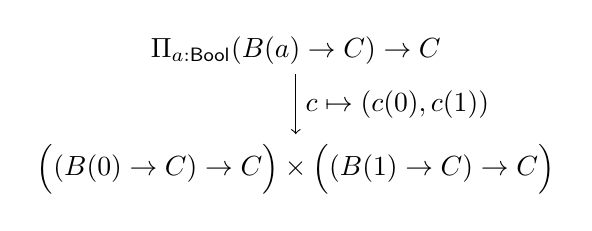
\begin{tikzpicture}
\node (N0) at (0,12) {$\prd{a:\Bool} (B(a) \to C) \to C$};
\node (N1) at (0,10.5) {$\Big((B(0) \to C) \to C\Big) \times \Big((B(1) \to C) \to C\Big)$};
\draw[->] (N0) -- node[right]{$c \mapsto (c(0), c(1))$} (N1);
\end{tikzpicture}
\end{center}
Since $B(0) = 0$, the type $B(0) \to C$ is contractible, with center $\lam{b:B(0)} \abort(C,F \; b)$. We thus have an equivalence
\begin{center}
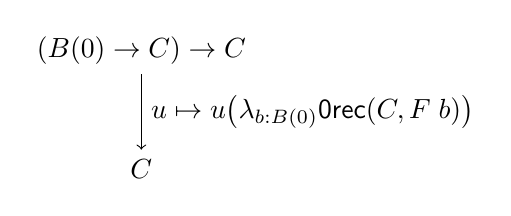
\begin{tikzpicture}
\node (N0) at (0,12) {$(B(0) \to C) \to C$};
\node (N1) at (0,10.5) {$C$};
\draw[->] (N0) -- node[right]{$u \mapsto u\big(\lam{b:B(0)} \abort(C,F \; b)\big)$} (N1);
\end{tikzpicture}
\end{center}
Since $B(1) = 1$, the map $x \mapsto \lam{\_}\; x$ is an equivalence from $C$ to $B(1) \to C$. Thus, we have an equivalence
\begin{center}
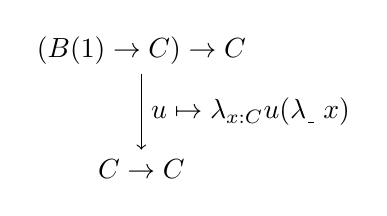
\begin{tikzpicture}
\node (N0) at (0,12) {$(B(1) \to C) \to C$};
\node (N1) at (0,10.5) {$C \to C$};
\draw[->] (N0) -- node[right]{$u \mapsto \lam{x:C} u(\lam{\_} \; x)$} (N1);
\end{tikzpicture}
\end{center}
Putting this all together, we see that the map 
\[ (C,c) \mapsto \Big(C,c\big(0,\lam{b} \abort(C,F \; b)\big),\lam{x:C} c(1, \lam{\_} \; x)\Big)\] 
is an equivalence from $\WAlg_{\UU_i}(A,B)$ to $\NatAlg_{\UU_i}$.
\end{proof}

\begin{lemma}
For any $\X : \WAlg_{\UU_i}(A,B)$ there is an equivalence
\[ \WFibAlgToNatFibAlg_{\UU_j} : \WFibAlg_{\UU_j}(A,B) \; \X \to \NatFibAlg_{\UU_j}(\WAlgToNatAlg_{\UU_i}(\X)) \]
\end{lemma}
\begin{proof}
Let an algebra $(C,c) : \WAlg_{\UU_i}(A,B)$ be given and fix $E : C \to \UU_j$. We have an equivalence
\begin{center}
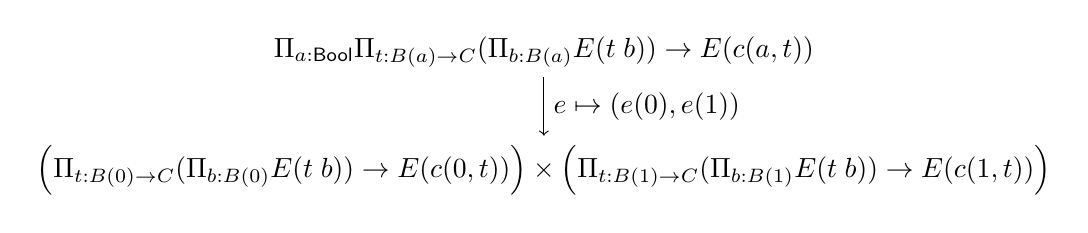
\begin{tikzpicture}
\node (N0) at (0,12) {$\prd{a:\Bool}\prd{t:B(a)\to C} (\prd{b:B(a)} E(t\;b)) \to E(c(a,t))$};
\node (N1) at (0,10.5) {$\Big(\prd{t:B(0)\to C} (\prd{b:B(0)} E(t\;b)) \to E(c(0,t))\Big) \times \Big(\prd{t:B(1)\to C} (\prd{b:B(1)} E(t\;b)) \to E(c(1,t))\Big)$};
\draw[->] (N0) -- node[right]{$e \mapsto (e(0), e(1))$} (N1);
\end{tikzpicture}
\end{center}
Since $B(0) = 0$, the type $B(0) \to C$ is contractible, with center $\lam{b:B(0)} \abort(C,F \; b)$. Likewise, $\prd{b:B(0)} E(\abort(C,F \; b))$ is contractible, with center 
$\lam{b:B(0)} \abort\big(E(\abort(C,F \; b)), F \;b\big)$. We thus have equivalences
\begin{center}
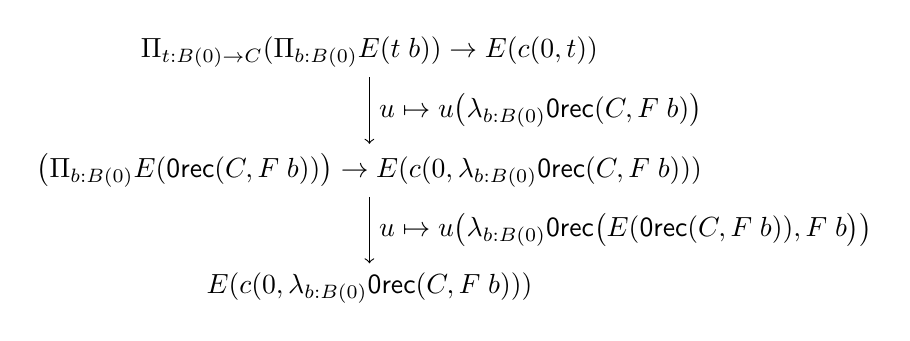
\begin{tikzpicture}
\node (N0) at (0,12) {$\prd{t:B(0)\to C} (\prd{b:B(0)} E(t\;b)) \to E(c(0,t))$};
\node (N1) at (0,10.5) {$\big(\prd{b:B(0)} E(\abort(C,F \; b))\big) \to E(c(0,\lam{b:B(0)} \abort(C,F \; b)))$};
\node (N2) at (0,9) {$E(c(0,\lam{b:B(0)} \abort(C,F \; b)))$};
\draw[->] (N0) -- node[right]{$u \mapsto u\big(\lam{b:B(0)} \abort(C,F \; b)\big)$} (N1);
\draw[->] (N1) -- node[right]{$u \mapsto u\big(\lam{b:B(0)} \abort\big(E(\abort(C,F \; b)), F \;b\big)\big)$} (N2);
\end{tikzpicture}
\end{center}
Since $B(1) = 1$, the map $x \mapsto \lam{\_}\; x$ is an equivalence from $C$ to $B(1) \to C$. Likewise, for any $x:C$ the map $y \mapsto \lam{\_}\; y$  is an equivalence from $E(x)$ to $B(1) \to E(x)$. Thus, we have equivalences
\begin{center}
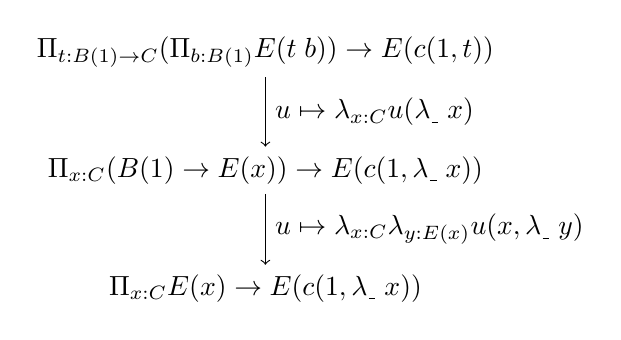
\begin{tikzpicture}
\node (N0) at (0,12) {$\prd{t:B(1)\to C} (\prd{b:B(1)} E(t\;b)) \to E(c(1,t))$};
\node (N1) at (0,10.5) {$\prd{x:C} (B(1) \to E(x)) \to E(c(1,\lam{\_} \; x))$};
\node (N2) at (0,9) {$\prd{x:C} E(x) \to E(c(1,\lam{\_} \; x))$};
\draw[->] (N0) -- node[right]{$u \mapsto \lam{x:C} u(\lam{\_} \; x)$} (N1);
\draw[->] (N1) -- node[right]{$u \mapsto \lam{x:C} \lam{y:E(x)} u(x,\lam{\_} \; y)$} (N2);
\end{tikzpicture}
\end{center}
Putting this all together, we see that the map 
\[ (E,e) \mapsto \Big(E,e\big(0,\lam{b} \abort(C,F \; b), \lam{b} \abort(E(\abort(C,F \; b)), F \;b)\big),\lam{x:C} \lam{y:E(x)} e(1, \lam{\_} \; x, \lam{\_} \; y)\Big)\] 
is an equivalence from $\WFibAlg_{\UU_j}(A,B) \; (C,c)$ to $\NatFibAlg_{\UU_j}(\WAlgToNatAlg_{\UU_i} \; (C,c))$.
\end{proof}

\begin{lemma}
For any $\X : \WAlg_{\UU_i}(A,B)$ and $\Y : \WFibAlg_{\UU_j}(A,B) \; \X$ we have
\[ \WFibHom \; \X \; \Y \;\; \simeq \;\; \NatFibHom \; \big(\WAlgToNatAlg_{\UU_i}(\X)\big) \; \big(\WFibAlgToNatFibAlg_{\UU_j}(\Y)\big) \]
\end{lemma}
\begin{proof}
Let algebras $(C,c) : \WAlg_{\UU_i}(A,B)$ and $(E,e) : \WFibAlg_{\UU_j}(A,B) \; (C,c)$ be given and fix $f : \prd{x:C} E(x)$. We have an equivalence
\begin{center}
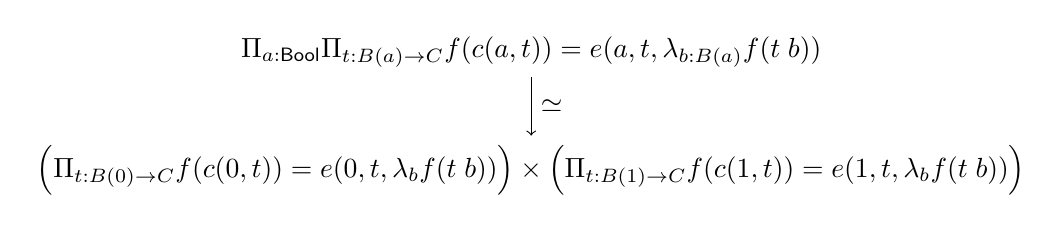
\begin{tikzpicture}
\node (N0) at (0,12) {$\prd{a:\Bool}\prd{t:B(a)\to C} f(c(a,t)) = e(a,t,\lam{b:B(a)} f(t\;b))$};
\node (N1) at (0,10.5) {$\Big(\prd{t:B(0)\to C} f(c(0,t)) = e(0,t,\lam{b} f(t\;b))\Big) \times \Big(\prd{t:B(1)\to C} f(c(1,t)) = e(1,t,\lam{b} f(t\;b))\Big)$};
\draw[->] (N0) -- node[right]{$\simeq$} (N1);
\end{tikzpicture}
\end{center}
Since $B(0) = 0$, the type $B(0) \to C$ is contractible, with center $\lam{b:B(0)} \abort(C,F \; b)$. Furthermore, since all functions out of $\zero$ are equal, we have
\[\lam{b} f(\abort(C,F \; b)) = \lam{b} \abort(E(\abort(C,F \; b)), F \;b)\] This implies the following equivalences:
\begin{center}
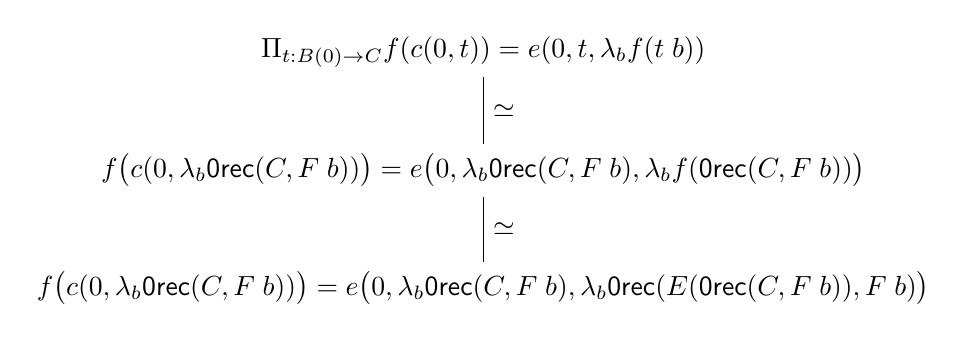
\begin{tikzpicture}
\node (N0) at (0,12) {$\prd{t:B(0)\to C} f(c(0,t)) = e(0,t,\lam{b} f(t\;b))$};
\node (N1) at (0,10.5) {$f\big(c(0,\lam{b} \abort(C,F \; b))\big) = e\big(0,\lam{b} \abort(C,F \; b),\lam{b} f(\abort(C,F \; b))\big)$};
\node (N2) at (0,9) {$f\big(c(0,\lam{b} \abort(C,F \; b))\big) = e\big(0,\lam{b} \abort(C,F \; b),\lam{b} \abort(E(\abort(C,F \; b)), F \;b)\big)$};
\draw[-] (N0) -- node[right]{$\simeq$} (N1);
\draw[-] (N1) -- node[right]{$\simeq$} (N2);
\end{tikzpicture}
\end{center}
Since $B(1) = 1$, the map $x \mapsto \lam{\_}\; x$ is an equivalence from $C$ to $B(1) \to C$. Thus, we have an equivalence
\begin{center}
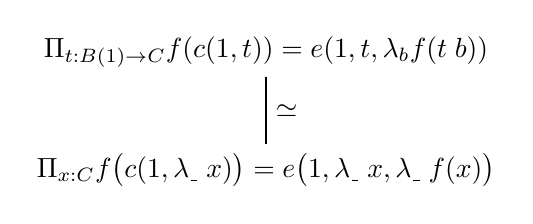
\begin{tikzpicture}
\node (N0) at (0,12) {$\prd{t:B(1)\to C} f(c(1,t)) = e(1,t,\lam{b} f(t\;b))$};
\node (N1) at (0,10.5) {$\prd{x:C} f\big(c(1,\lam{\_} \; x)\big) = e\big(1,\lam{\_} \; x,\lam{\_} \; f(x)\big)$};
\draw[-] (N0) -- node[right]{$\simeq$} (N1);
\end{tikzpicture}
\end{center}
This finishes the proof.
\end{proof}

\begin{corollary}
For any $\X : \WAlg_{\UU_i}(A,B)$ and $\Y : \WAlg_{\UU_j}(A,B)$ we have
\[ \WHom \; \X \; \Y \;\; \simeq \;\; \NatHom \; \big(\WAlgToNatAlg_{\UU_i}(\X)\big) \; \big(\WAlgToNatAlg_{\UU_j}(\Y)\big) \]
\end{corollary}

\begin{corollary}
For any $\X : \NatAlg_{\UU_i}$ we have
\begin{alignat*}{4}
& \HasNatRec_{\UU_j}(\X) & \;\; \simeq \;\; & \HasWRec_{\UU_j}(\WAlgToNatAlg_{\UU_i}^{-1}(\X)) \\
& \HasNatInd_{\UU_j}(\X) & \;\; \simeq \;\; & \HasWInd_{\UU_j}(\WAlgToNatAlg_{\UU_i}^{-1}(\X)) \\
& \HasNatRecUniq_{\UU_j}(\X) &  \simeq \;\; & \HasWRecUniq_{\UU_j}(\WAlgToNatAlg_{\UU_i}^{-1}(\X)) \\
& \HasNatIndUniq_{\UU_j}(\X) & \simeq \;\; &  \HasWIndUniq_{\UU_j}(\WAlgToNatAlg_{\UU_i}^{-1}(\X)) \\
& \IsNatHInit_{\UU_j}(\X) & \simeq \;\; & \IsWHInit_{\UU_j}(\WAlgToNatAlg_{\UU_i}^{-1}(\X))
\end{alignat*}
\end{corollary}

\begin{corollary}\label{lem:NatMainInt}
In $\Hint$, the following conditions on an algebra $\X : \NatAlg_{\UU_i}$ are equivalent:
\begin{enumerate}
\item $\X$ satisfies the induction principle on the universe $\UU_j$
\item $\X$ satisfies the recursion and recursion uniqueness principles on the universe $\UU_j$
\item $\X$ is homotopy-initial on the universe $\UU_j$  
\end{enumerate}
for $j \geq i$. In other words, we have \[ \HasNatInd_{\UU_j}(\X)  \;\; \simeq \;\; \HasNatRec_{\UU_j}(\X) \times \HasNatRecUniq_{\UU_j}(\X) \;\; \simeq \;\; \IsNatHInit_{\UU_j}(\X) \]
provided $j \geq i$. Furthermore, all 3 conditions are mere propositions.
\end{corollary}

We can thus characterize the type $\nat$ using the universal property of initiality as follows.
\begin{corollary}\label{lem:NatInitInt}
In $\Hint$ with natural numbers, the algebra $(\nat,\z,\suc(-)) : \NatAlg_{\UU_0}$ is homotopy-initial on any universe $\UU_j$.
\end{corollary}

\begin{corollary}\label{lem:NatCharInt}
In $\Hint$ extended with an algebra $\X : \NatAlg_{\UU_0}$ which is homotopy-initial on any universe $\UU_j$, the type $\nat$ with propositional computation rules is definable. 
\end{corollary}
\begin{proof}
We have an algebra $\cdot \vdash \X : \NatAlg_{\UU_0}$ such that for any $j$, there exists a term $\cdot \vdash h_j  : \IsNatHInit_{\UU_j}(\X)$. Since the requirement $j \geq 0$ always holds, Cor.~\ref{lem:NatMainInt} implies that for any $j$, we have a term $\cdot \vdash r_j : \HasNatInd_{\UU_j}(\X)$. This implies that the type $\nat$ with propositional computation rules is definable.
\end{proof}






\subsection*{Acknowledgements}

We would like to thank Vladimir Voevodsky and Michael Warren for helpful discussions
on the subject of this paper. In particular, Vladimir Voevodsky suggested a simplification of the 
proof that the rules for homotopical W-types imply h-initiality.

Steve Awodey gratefully acknowledges the support of the National Science Foundation, Grant DMS-1001191
 and the Air Force OSR, Grant 11NL035.
Nicola Gambino is grateful for the support of the Institute for Advanced Study, where
he worked on this project. This work was supported by the National Science Foundation 
under agreement No.\ DMS-0635607. Any opinions, findings and conclusions or recommendations
expressed in this material are those of the authors and do not necessarily reflect the views of
the National Science Foundation.
Kristina Sojakova is grateful for the support of CyLab at Carnegie
Mellon under grants DAAD19-02-1-0389 and W911NF-09-1-0273 from the Army
Research Office.



\bibliographystyle{plain}

\bibliography{references}
                        


\end{document}